\documentclass[a4paper, 14pt]{extarticle}

% Поля
%--------------------------------------
\usepackage{geometry}
\geometry{a4paper,tmargin=2cm,bmargin=2cm,lmargin=3cm,rmargin=1cm}
%--------------------------------------


%Russian-specific packages
%--------------------------------------
\usepackage[T2A]{fontenc}
\usepackage[utf8]{inputenc} 
\usepackage[english, main=russian]{babel}
%--------------------------------------

\usepackage{textcomp}

% Красная строка
%--------------------------------------
\usepackage{indentfirst}               
%--------------------------------------             


%Graphics
%--------------------------------------
\usepackage{graphicx}
\graphicspath{ {./images/} }
\usepackage{wrapfig}
%--------------------------------------

% Полуторный интервал
%--------------------------------------
\linespread{1.3}                    
%--------------------------------------

%Выравнивание и переносы
%--------------------------------------
% Избавляемся от переполнений
\sloppy
% Запрещаем разрыв страницы после первой строки абзаца
\clubpenalty=10000
% Запрещаем разрыв страницы после последней строки абзаца
\widowpenalty=10000
%--------------------------------------

%Списки
\usepackage{enumitem}

%Подписи
\usepackage{caption} 

\newenvironment{longlisting}{\captionsetup{type=listing}}{}

%Гиперссылки
\usepackage{hyperref}

\hypersetup{
  colorlinks=true,
  unicode=true,
}

%Рисунки
%--------------------------------------
\DeclareCaptionLabelSeparator*{emdash}{~--- }
\captionsetup[figure]{labelsep=emdash,font=onehalfspacing,position=bottom}
%--------------------------------------

\usepackage{tempora}

%Листинги
%--------------------------------------
\usepackage{minted}

\renewcommand\listingscaption{Листинг}
\setminted[cpp]{
  frame=single,
  fontsize=\small,
  linenos,
  xleftmargin=1.5em,
}
%--------------------------------------

%%% Математические пакеты %%%
%--------------------------------------
\usepackage{amsthm,amsfonts,amsmath,amssymb,amscd}  % Математические дополнения от AMS
\usepackage{mathtools}                              % Добавляет окружение multlined
\usepackage[perpage]{footmisc}
%--------------------------------------

%--------------------------------------
%			НАЧАЛО ДОКУМЕНТА
%--------------------------------------

\begin{document}

%--------------------------------------
%			ТИТУЛЬНЫЙ ЛИСТ
%--------------------------------------
\begin{titlepage}
\thispagestyle{empty}
\newpage


%Шапка титульного листа
%--------------------------------------
\vspace*{-60pt}
\hspace{-65pt}
\begin{minipage}{0.3\textwidth}
\hspace*{-20pt}\centering

\includegraphics[width=\textwidth]{emblem}
\end{minipage}
\begin{minipage}{0.67\textwidth}\small \textbf{
\vspace*{-0.7ex}
\hspace*{-6pt}\centerline{Министерство науки и высшего образования Российской Федерации}
\vspace*{-0.7ex}
\centerline{Федеральное государственное бюджетное образовательное учреждение }
\vspace*{-0.7ex}
\centerline{высшего образования}
\vspace*{-0.7ex}
\centerline{<<Московский государственный технический университет}
\vspace*{-0.7ex}
\centerline{имени Н.Э. Баумана}
\vspace*{-0.7ex}
\centerline{(национальный исследовательский университет)>>}
\vspace*{-0.7ex}
\centerline{(МГТУ им. Н.Э. Баумана)}}
\end{minipage}
%--------------------------------------

%Полосы
%--------------------------------------
\vspace{-25pt}
\hspace{-35pt}\rule{\textwidth}{2.3pt}

\vspace*{-20.3pt}
\hspace{-35pt}\rule{\textwidth}{0.4pt}
%--------------------------------------

\vspace{1.5ex}
\hspace{-35pt} \noindent \small ФАКУЛЬТЕТ\hspace{80pt} <<Информатика и системы управления>>

\vspace*{-16pt}
\hspace{47pt}\rule{0.83\textwidth}{0.4pt}

\vspace{0.5ex}
\hspace{-35pt} \noindent \small КАФЕДРА\hspace{50pt} <<Теоретическая информатика и компьютерные технологии>>

\vspace*{-16pt}
\hspace{30pt}\rule{0.866\textwidth}{0.4pt}
  
\vspace{11em}

\begin{center}
\Large {\bf Домашняя работа № 2} \\ 
\large {\bf по курсу <<Теория искусственных нейронных сетей>>} \\
\large <<Разработка многослойного персептрона на основе обратного распространения ошибки FFNN>> 
\end{center}\normalsize

\vspace{8em}


\begin{flushright}
  {Студент группы ИУ9-71Б Афанасьев И. \hspace*{15pt}\\ 
  \vspace{2ex}
  Преподаватель Каганов Ю. Т.\hspace*{15pt}}
\end{flushright}

\bigskip

\vfill
 

\begin{center}
\textsl{Москва 2024}
\end{center}
\end{titlepage}
%--------------------------------------
%		КОНЕЦ ТИТУЛЬНОГО ЛИСТА
%--------------------------------------

\renewcommand{\ttdefault}{pcr}

\setlength{\tabcolsep}{3pt}
\newpage
\setcounter{page}{2}

\section{Цель работы}

\begin{enumerate}
  \item Изучение многослойного персептрона, исследование его работы на основе использования градиентного метода оптимизации и различных целевых функций.
\end{enumerate}

\section{Постановка задачи}

\begin{enumerate}
  \item Реализовать на языке высокого уровня многослойный персептрон и проверить его работоспособность на примере данных, выбранных из MNIST dataset. 
  \item Исследовать работу персептрона на основе использования различных целевых функций (среднеквадратичная ошибка, перекрестная энтропия, дивергенция
    Кульбака-Лейблера).
  \item Провести исследование эффективности работы многослойного персептрона при изменении гиперпараметров (количества нейронов и количества слоев).
  \item Подготовить отчет с распечаткой текста программы, графиками результатов исследования и анализом результатов.
\end{enumerate}

\section{Реализация}

Каркас для обучения многослойного персептрона на основе стохастического градиентного спуска и обратного распространения ошибки был разработан в
домашнем задании №1. Программа написана на языке C++; для выполнения матричных операций используется библиотека
\href{https://eigen.tuxfamily.org/index.php?title=Main_Page}{Eigen}.

В листинге \ref{lst:activation_function.h} приводится реализация функций активации: линейной, ReLU, Leaky ReLU, сигмоиды, гиперболического
тангенса и Softmax.

В листинге \ref{lst:cost_function.h} приводится реализация функций ошибки: MSE, кросс-энтропии и дивергенции Кульбака-Лейблера.

В листингах \ref{lst:perceptron.h} и \ref{lst:perceptron.cc} приводится реализация многослойного персептрона и его обучения.

В листингах \ref{lst:data_supplier.h} и \ref{lst:data_supplier.cc} приводится программный код формирования данных для обучения, валидации и
тестирования на основе исходных файлов датасета MNIST в формате CSV.

В листинге \ref{lst:main.cc} приводится \texttt{main}-файл с различными конфигурациями персептрона.
 
\begin{longlisting}
  \caption{Файл \texttt{activation\_function.h}}
  \inputminted{cpp}{../src/activation_function.h}
  \label{lst:activation_function.h}
\end{longlisting}

\begin{longlisting}
  \caption{Файл \texttt{cost\_function.h}}
  \inputminted{cpp}{../src/cost_function.h}
  \label{lst:cost_function.h}
\end{longlisting}

\begin{longlisting}
  \caption{Файл \texttt{perceptron.h}}
  \inputminted{cpp}{../src/perceptron.h}
  \label{lst:perceptron.h}
\end{longlisting}

\begin{longlisting}
  \caption{Файл \texttt{perceptron.cc}}
  \inputminted{cpp}{../src/perceptron.cc}
  \label{lst:perceptron.cc}
\end{longlisting}

\begin{longlisting}
  \caption{Файл \texttt{data\_supplier.h}}
  \inputminted{cpp}{../src/data_supplier.h}
  \label{lst:data_supplier.h}
\end{longlisting}

\begin{longlisting}
  \caption{Файл \texttt{data\_supplier.cc}}
  \inputminted{cpp}{../src/data_supplier.cc}
  \label{lst:data_supplier.cc}
\end{longlisting}

\begin{longlisting}
  \caption{Файл \texttt{main.cc}}
  \inputminted{cpp}{../src/main.cc}
  \label{lst:main.cc}
\end{longlisting}

\section{Результаты экспериментов}

На протяжении всех экспериментов значения некоторых гиперпараметров были фиксированными:
\begin{itemize}
  \item количество эпох: $200$;
  \item размер пакета данных (mini-batch) для стохастического градиентного спуска: $100$;
  \item коэффициент обучения (learning rate): $0.025$.
\end{itemize}
Изменялись значения следующих гиперпараметров:
\begin{itemize}
  \item количество скрытых слоёв: $1$ или $3$;
  \item количество нейронов в скрытых слоях: $20$ или $40$.
\end{itemize}
Таким образом, для каждой функции ошибки --- среднеквадратичной, перекрёстной энтропии и дивергенции Кульбака-Лейблера --- рассматривались четыре
конфигурации с разным числом скрытых слоёв и нейронов в них. В скрытых слоях всегда используется функция активации Leaky ReLU, на выходном слое ---
Softmax.

\subsection{Среднеквадратичная ошибка (MSE)}

\subsubsection{1 скрытый слой, 20 нейронов}

%  Epoch 199; training cost: 0.166286; training accuracy: 47518/50000; testing cost: 0.193274; testing accuracy: 9421/10000;

На рисунке\footnote{На некоторых рисунках шкала оси $Oy$ начинается с $0.2$, а не $0.0$.} \ref{fig:1_20_leaky_relu_softmax_mse_cost} изображено
изменение функции ошибки за период обучения персептрона. Здесь и далее график синей функции соответствует данным для обучения, график оранжевой
функции --- тестовым данным. В результате, ошибка на данных для обучения составляет $0.166286$, ошибка на тестовых данных --- $0.193274$.

\begin{figure}[!htb]
  \centering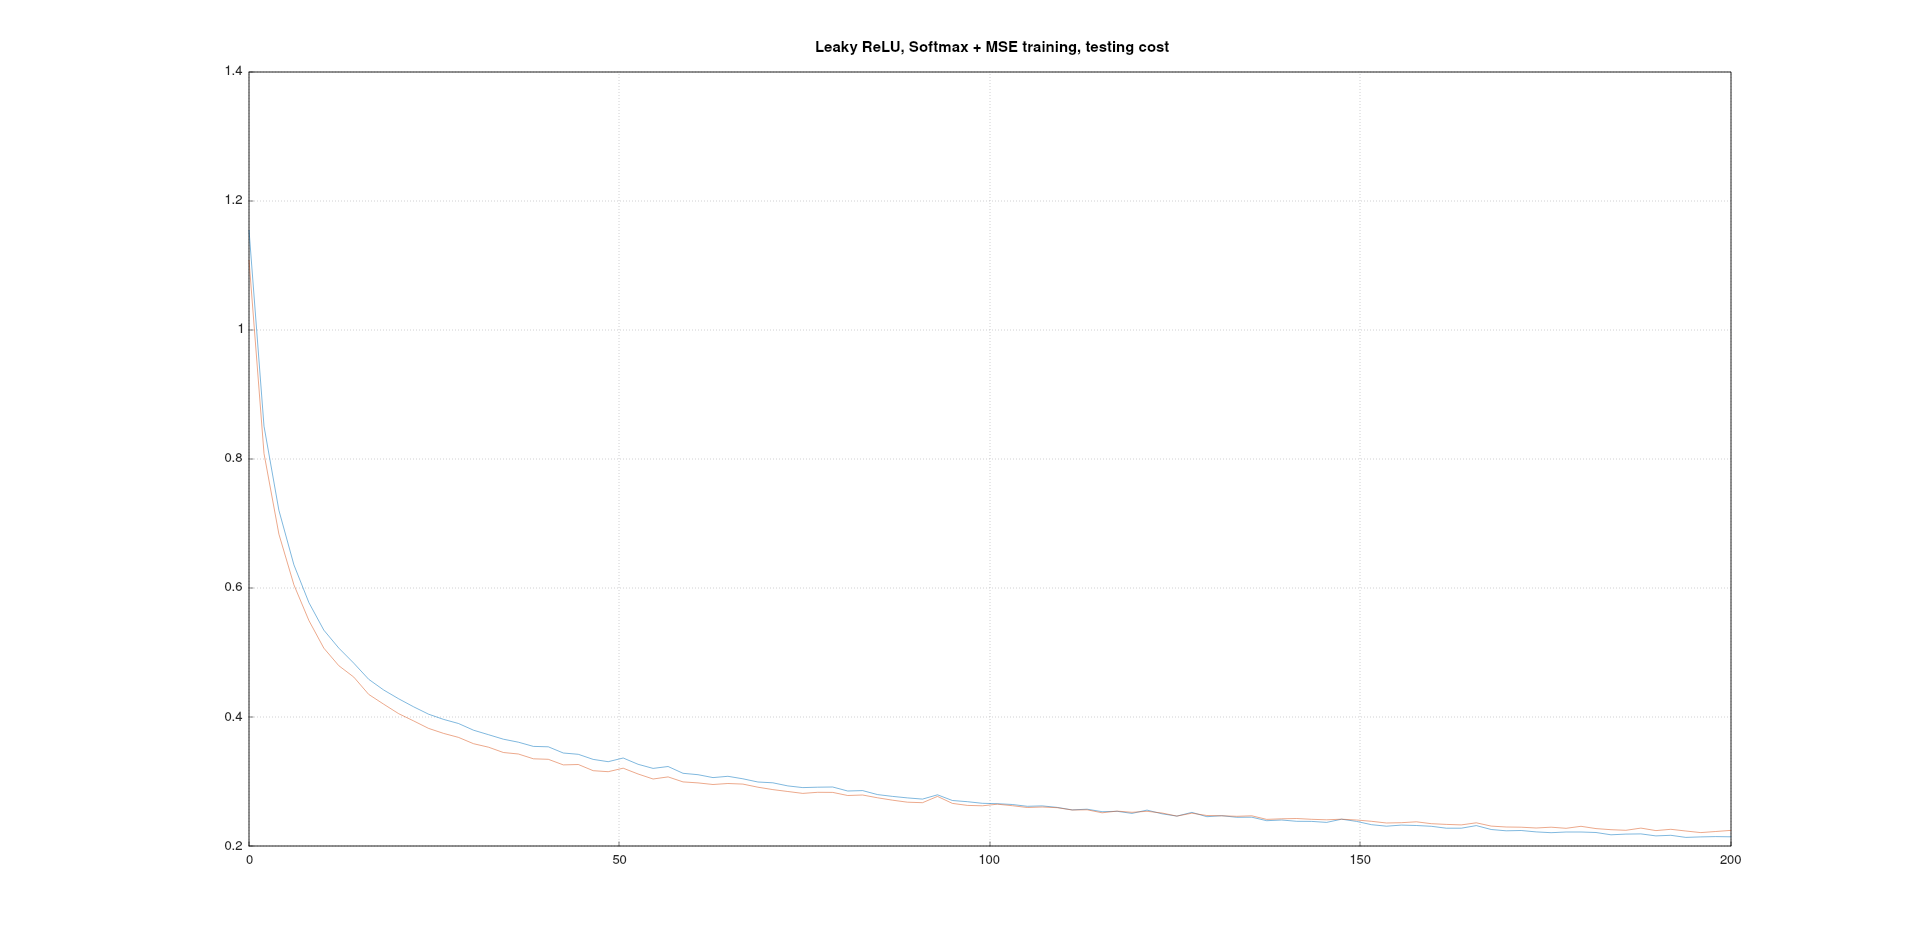
\includegraphics[width=\textwidth]{images/1_20_leaky_relu_softmax_mse_cost.png}
  \caption{}
  \label{fig:1_20_leaky_relu_softmax_mse_cost}
\end{figure}

На рисунке \ref{fig:1_20_leaky_relu_softmax_mse_accuracy} изображено изменение точности за период обучения персептрона.
В результате, точность на данных для обучения составляет $\frac{47518}{50000} \approx 95,04\%$, на тестовых данных --- $\frac{9421}{10000} = 94,21\%$.

\begin{figure}[!htb]
  \centering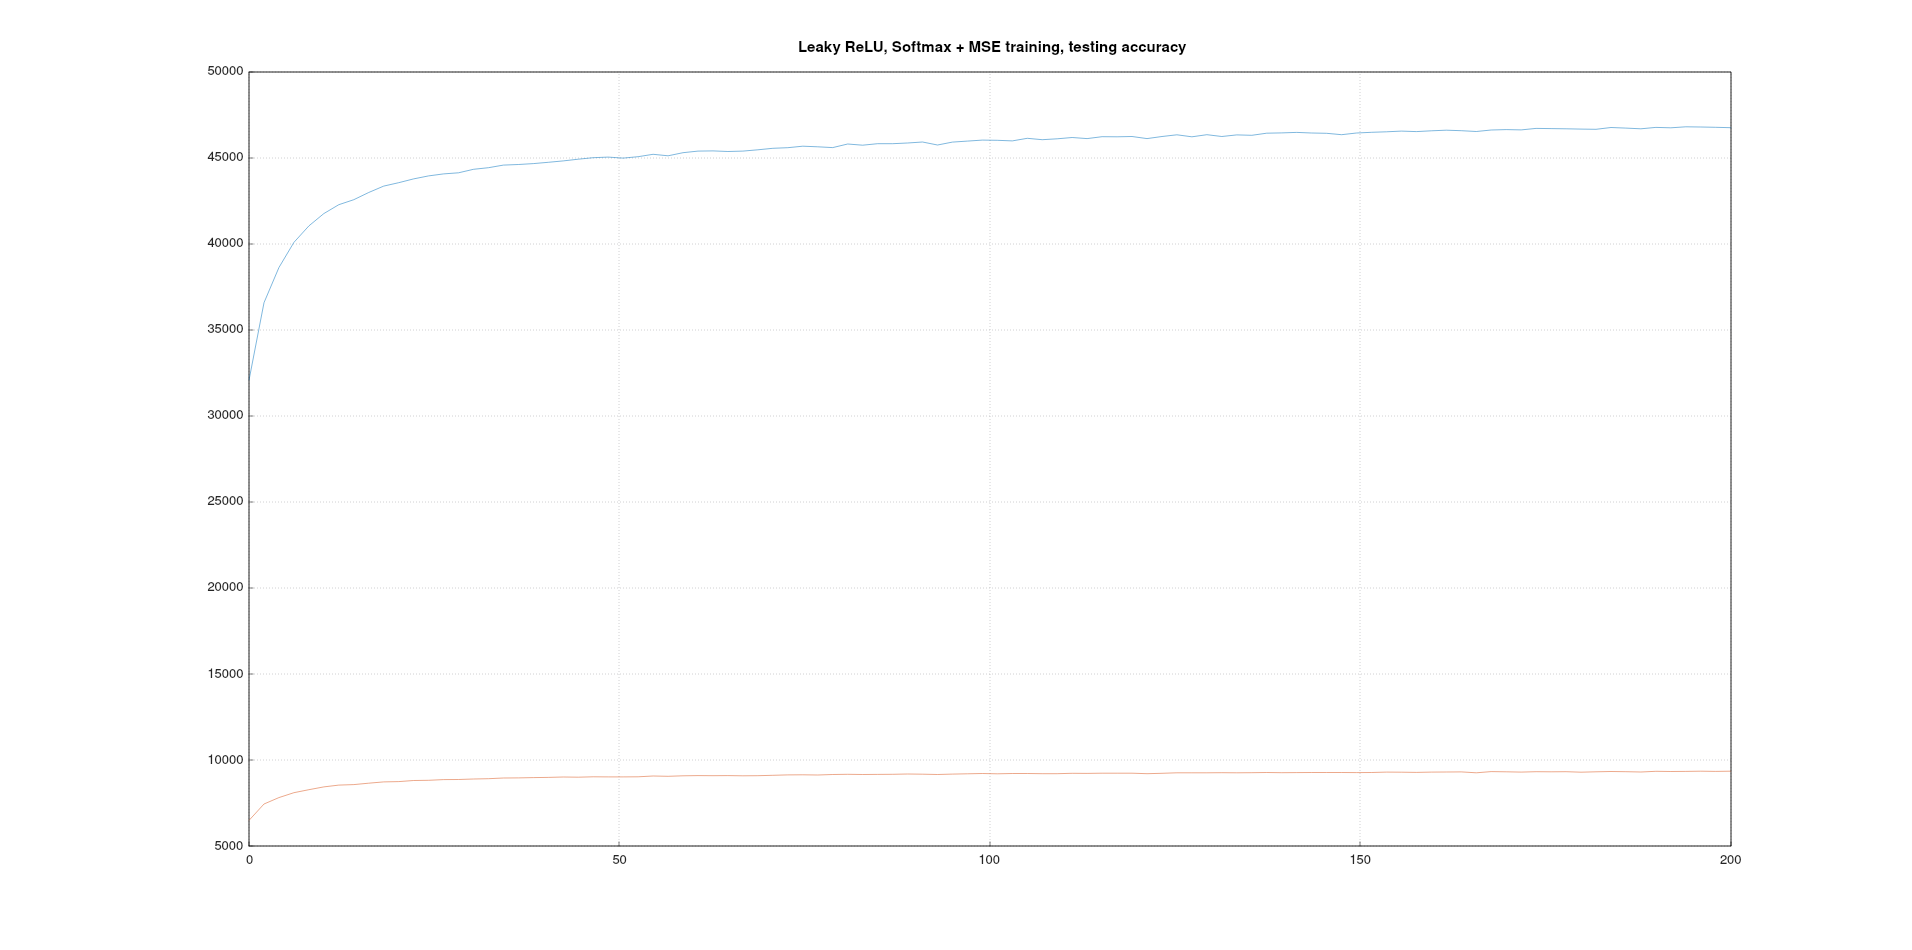
\includegraphics[width=\textwidth]{images/1_20_leaky_relu_softmax_mse_accuracy.png}
  \caption{}
  \label{fig:1_20_leaky_relu_softmax_mse_accuracy}
\end{figure}

\subsubsection{1 скрытый слой, 40 нейронов}

%  Epoch 199; training cost: 0.123245; training accuracy: 48121/50000; testing cost: 0.161724; testing accuracy: 9527/10000;

На рисунке \ref{fig:1_40_leaky_relu_softmax_mse_cost} изображено изменение функции ошибки за период обучения персептрона.
В результате, ошибка на данных для обучения составляет $0.123245$, ошибка на тестовых данных --- $0.161724$.

\begin{figure}[!htb]
  \centering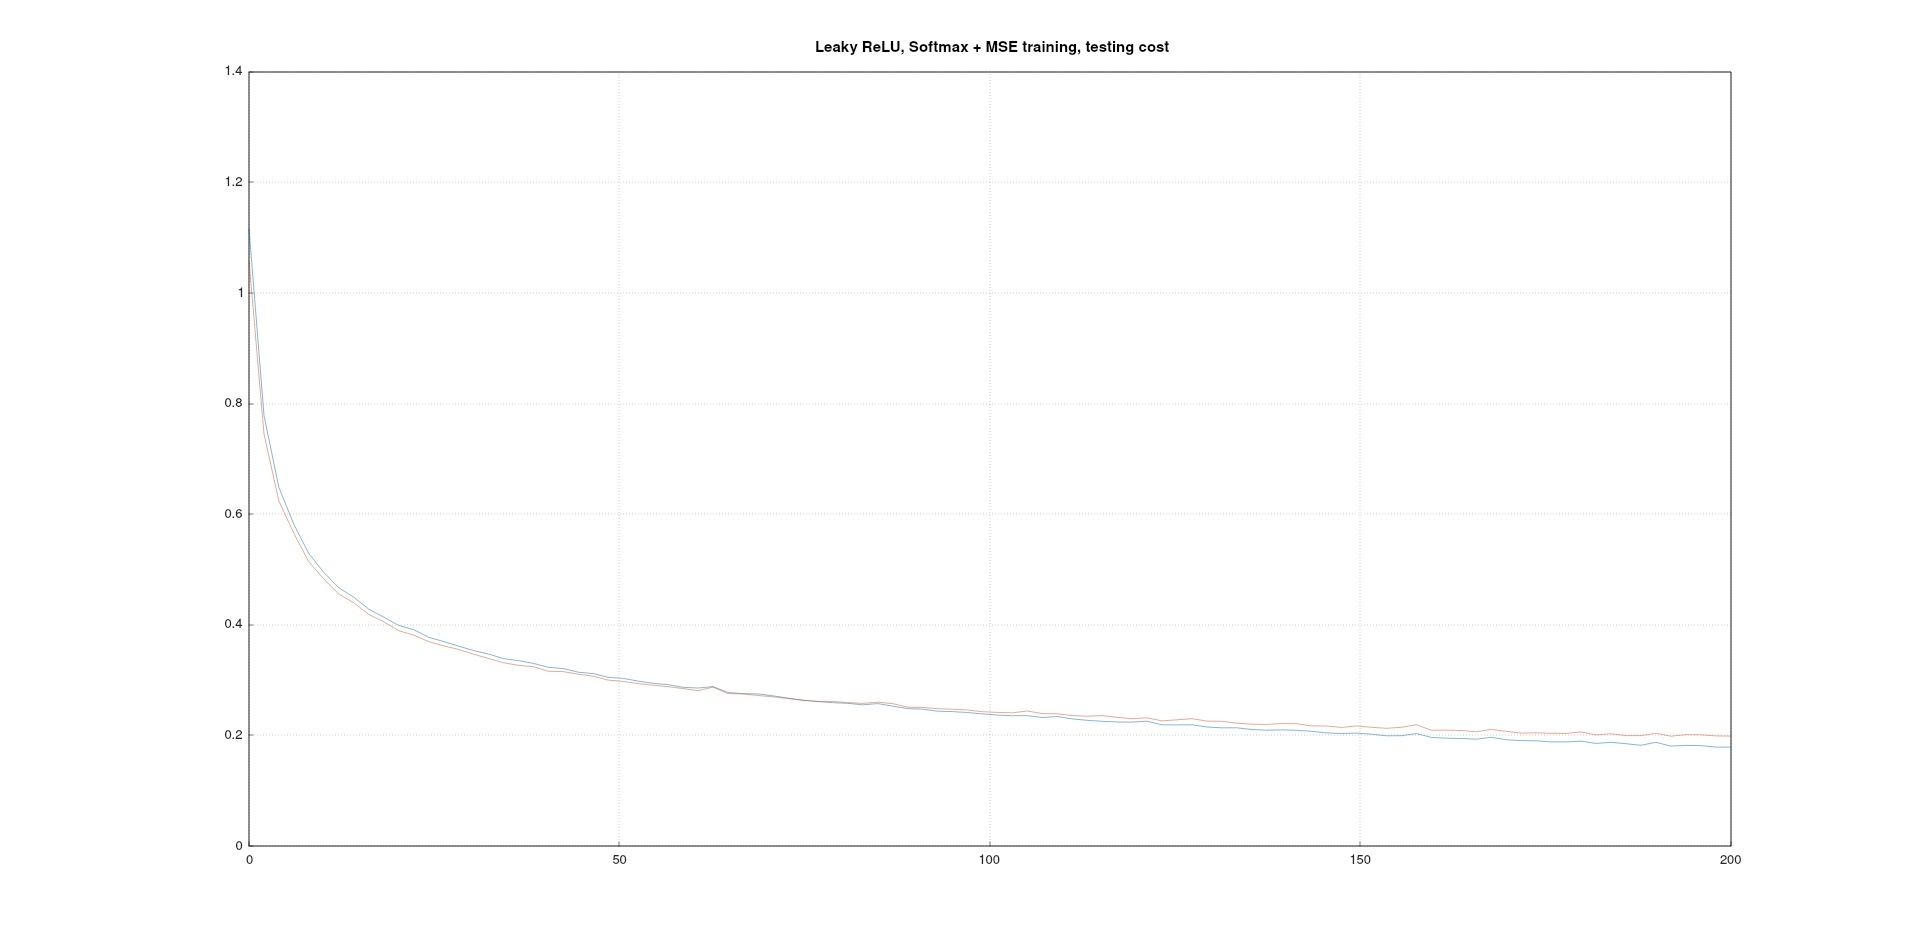
\includegraphics[width=\textwidth]{images/1_40_leaky_relu_softmax_mse_cost.png}
  \caption{}
  \label{fig:1_40_leaky_relu_softmax_mse_cost}
\end{figure}

На рисунке \ref{fig:1_40_leaky_relu_softmax_mse_accuracy} изображено изменение точности за период обучения персептрона.
В результате, точность на данных для обучения составляет $\frac{48121}{50000} \approx 96,24\%$, на тестовых данных --- $\frac{9527}{10000} = 95,27\%$.

\begin{figure}[!htb]
  \centering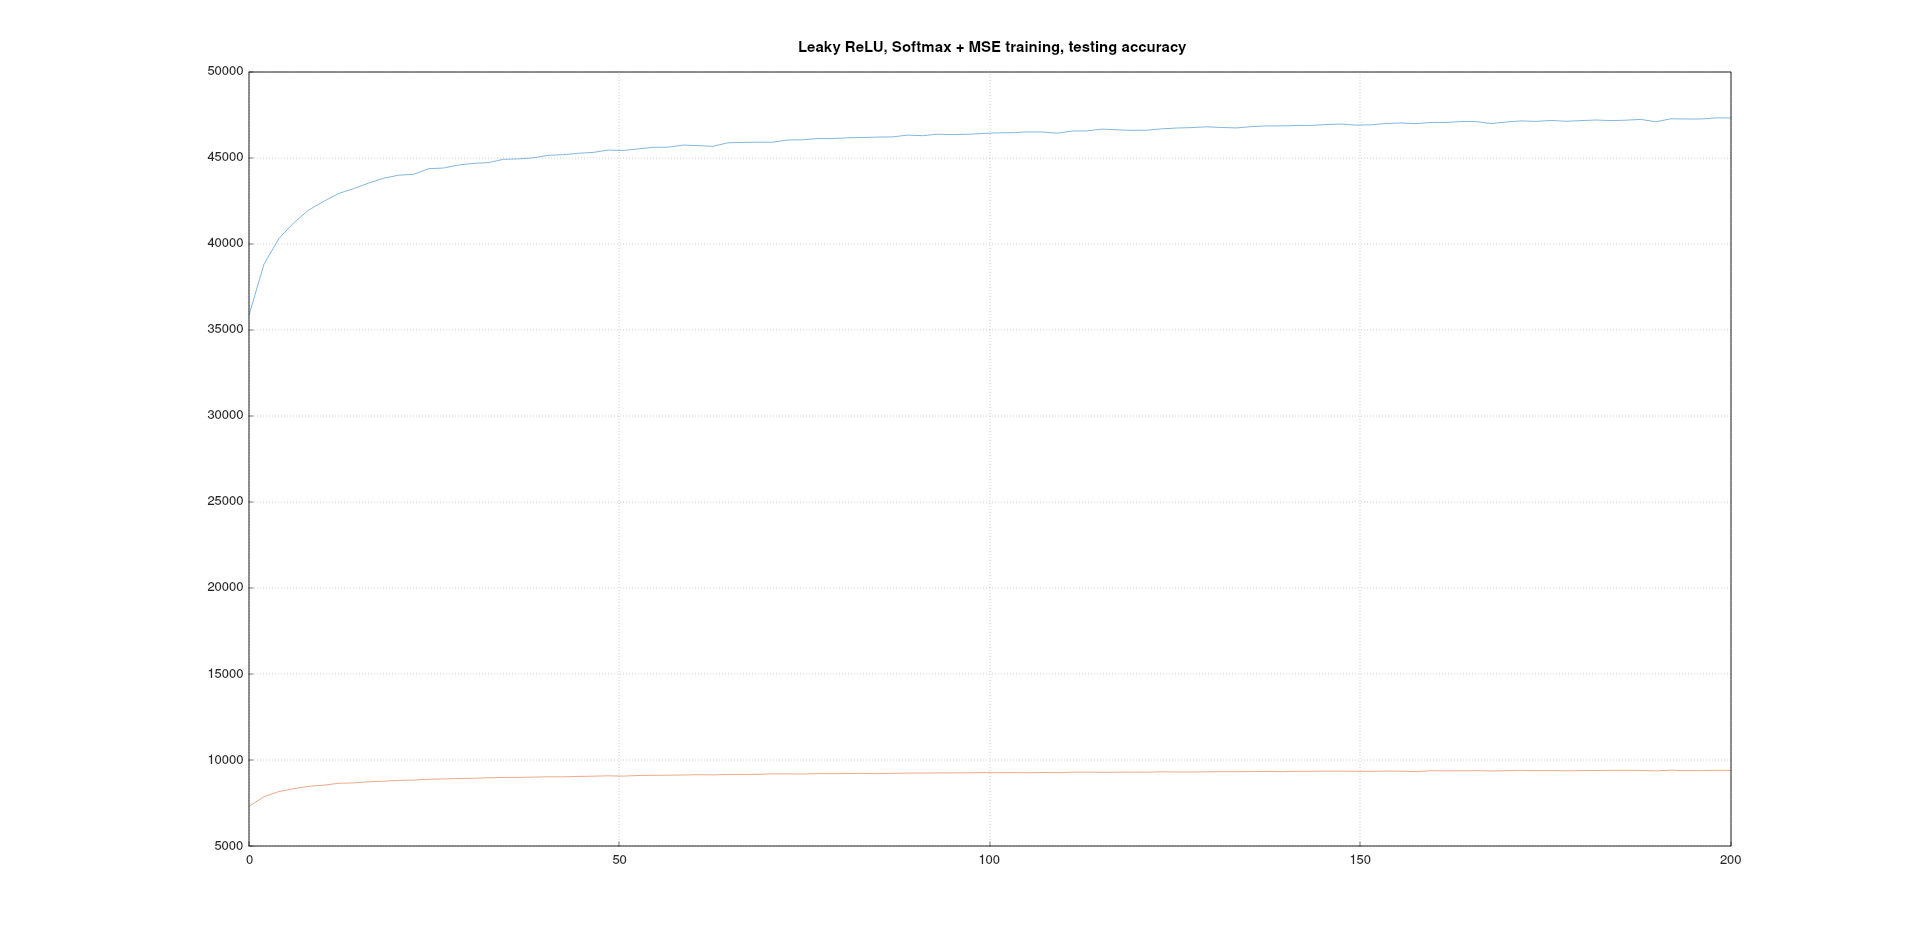
\includegraphics[width=\textwidth]{images/1_40_leaky_relu_softmax_mse_accuracy.png}
  \caption{}
  \label{fig:1_40_leaky_relu_softmax_mse_accuracy}
\end{figure}

\subsubsection{3 скрытых слоя, 20 нейронов}

%  Epoch 199; training cost: 0.163502; training accuracy: 47504/50000; testing cost: 0.206251; testing accuracy: 9416/10000;

На рисунке \ref{fig:3_20_leaky_relu_softmax_mse_cost} изображено изменение функции ошибки за период обучения персептрона.
В результате, ошибка на данных для обучения составляет $0.163502$, ошибка на тестовых данных --- $0.206251$.

\begin{figure}[!htb]
  \centering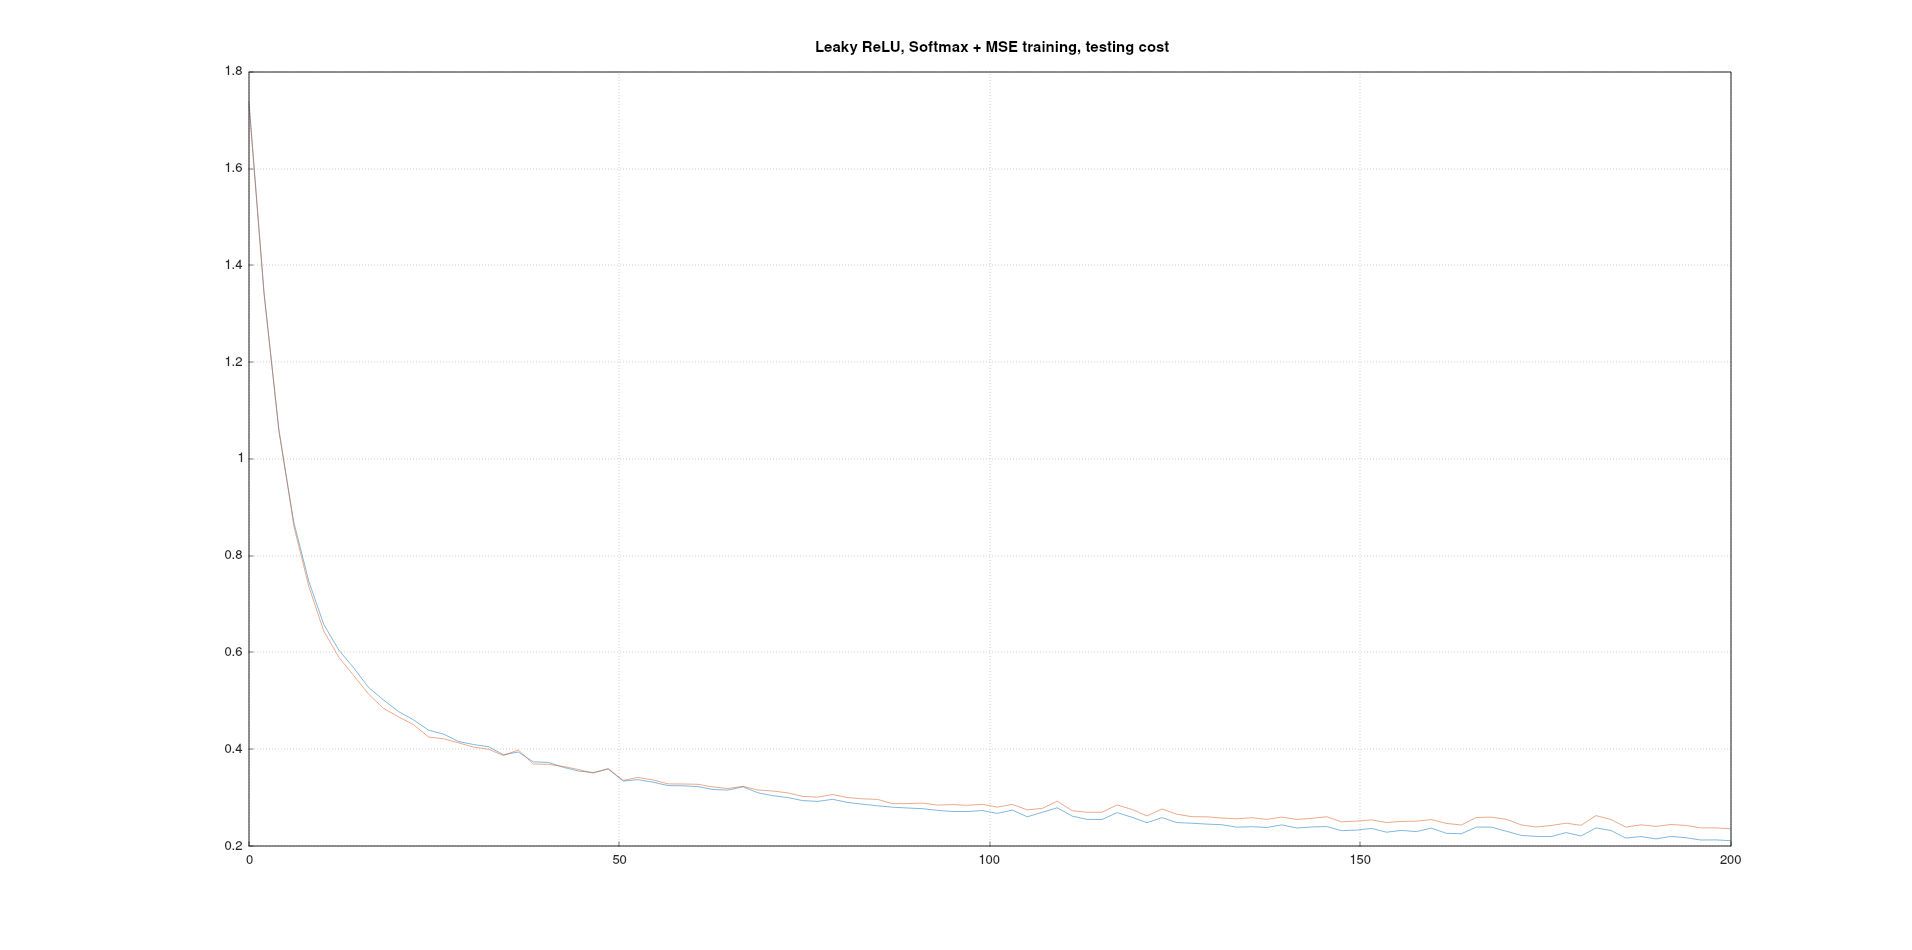
\includegraphics[width=\textwidth]{images/3_20_leaky_relu_softmax_mse_cost.png}
  \caption{}
  \label{fig:3_20_leaky_relu_softmax_mse_cost}
\end{figure}

На рисунке \ref{fig:3_20_leaky_relu_softmax_mse_accuracy} изображено изменение точности за период обучения персептрона.
В результате, точность на данных для обучения составляет $\frac{47504}{50000} \approx 95,01\%$, на тестовых данных --- $\frac{9416}{10000} = 94,16\%$.

\begin{figure}[!htb]
  \centering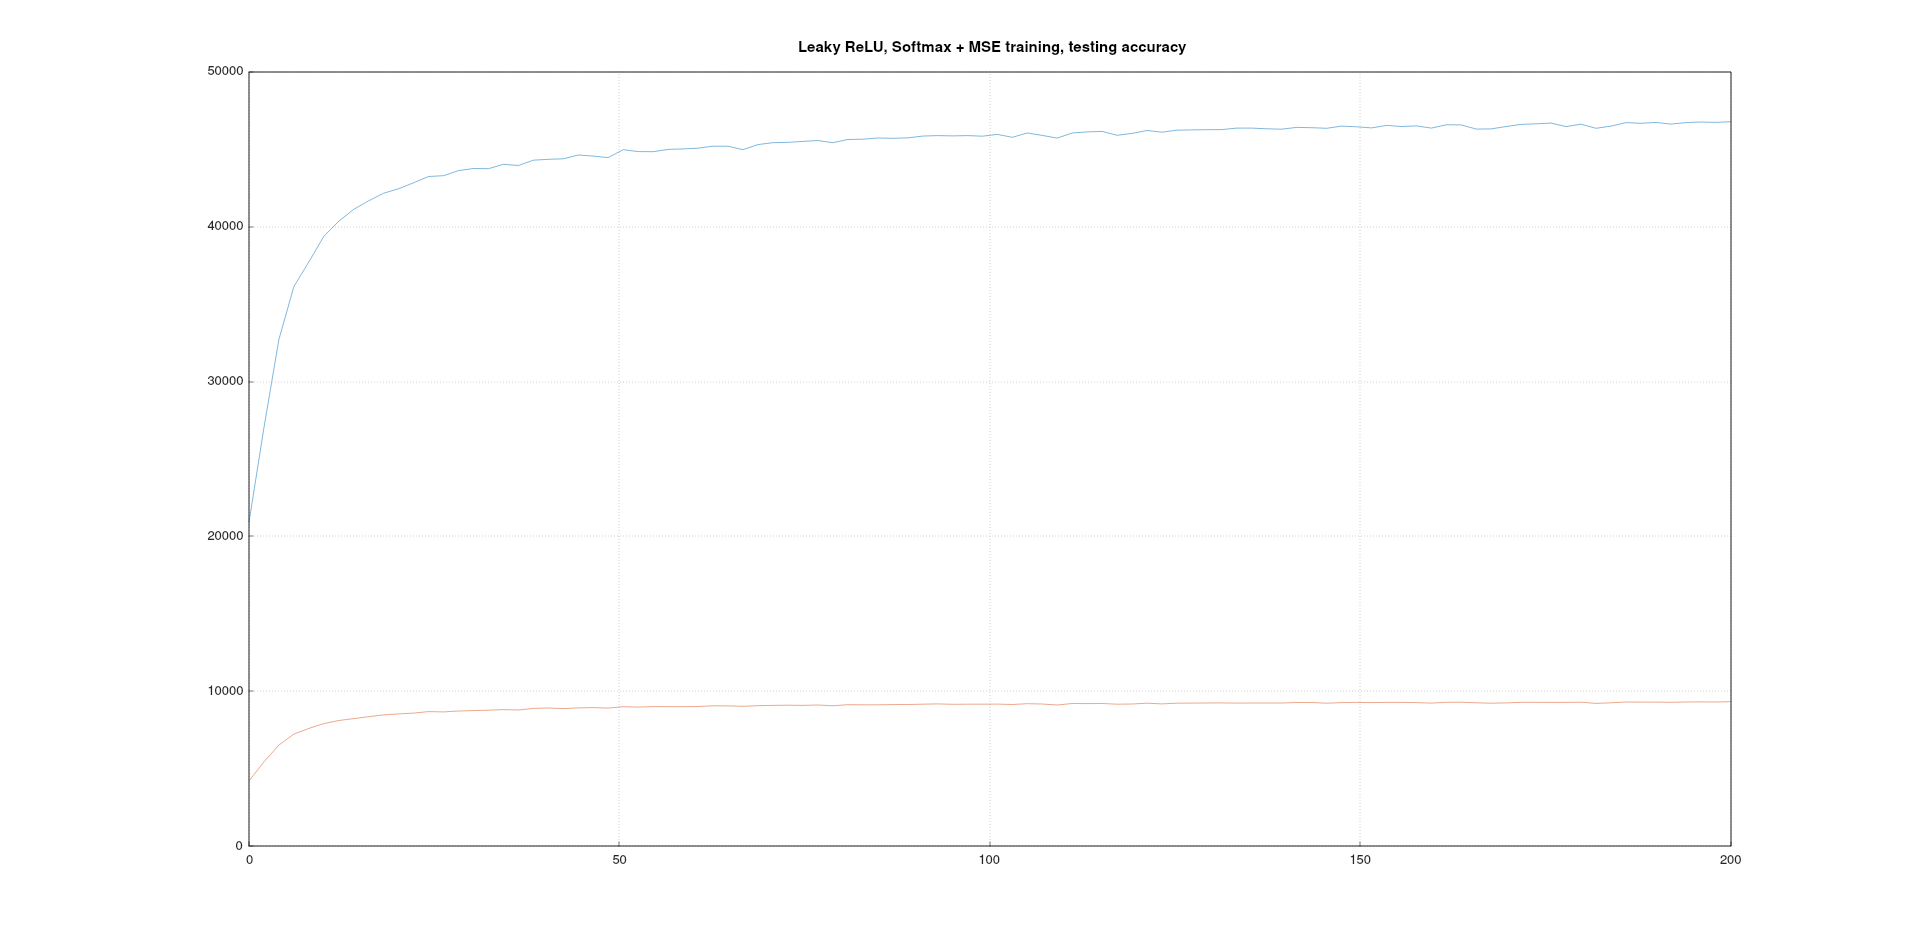
\includegraphics[width=\textwidth]{images/3_20_leaky_relu_softmax_mse_accuracy.png}
  \caption{}
  \label{fig:3_20_leaky_relu_softmax_mse_accuracy}
\end{figure}

\subsubsection{3 скрытых слоя, 40 нейронов}

%  Epoch 199; training cost: 0.105351; training accuracy: 48422/50000; testing cost: 0.190718; testing accuracy: 9481/10000;

На рисунке \ref{fig:3_40_leaky_relu_softmax_mse_cost} изображено изменение функции ошибки за период обучения персептрона.
В результате, ошибка на данных для обучения составляет $0.105351$, ошибка на тестовых данных --- $0.190718$.

\begin{figure}[!htb]
  \centering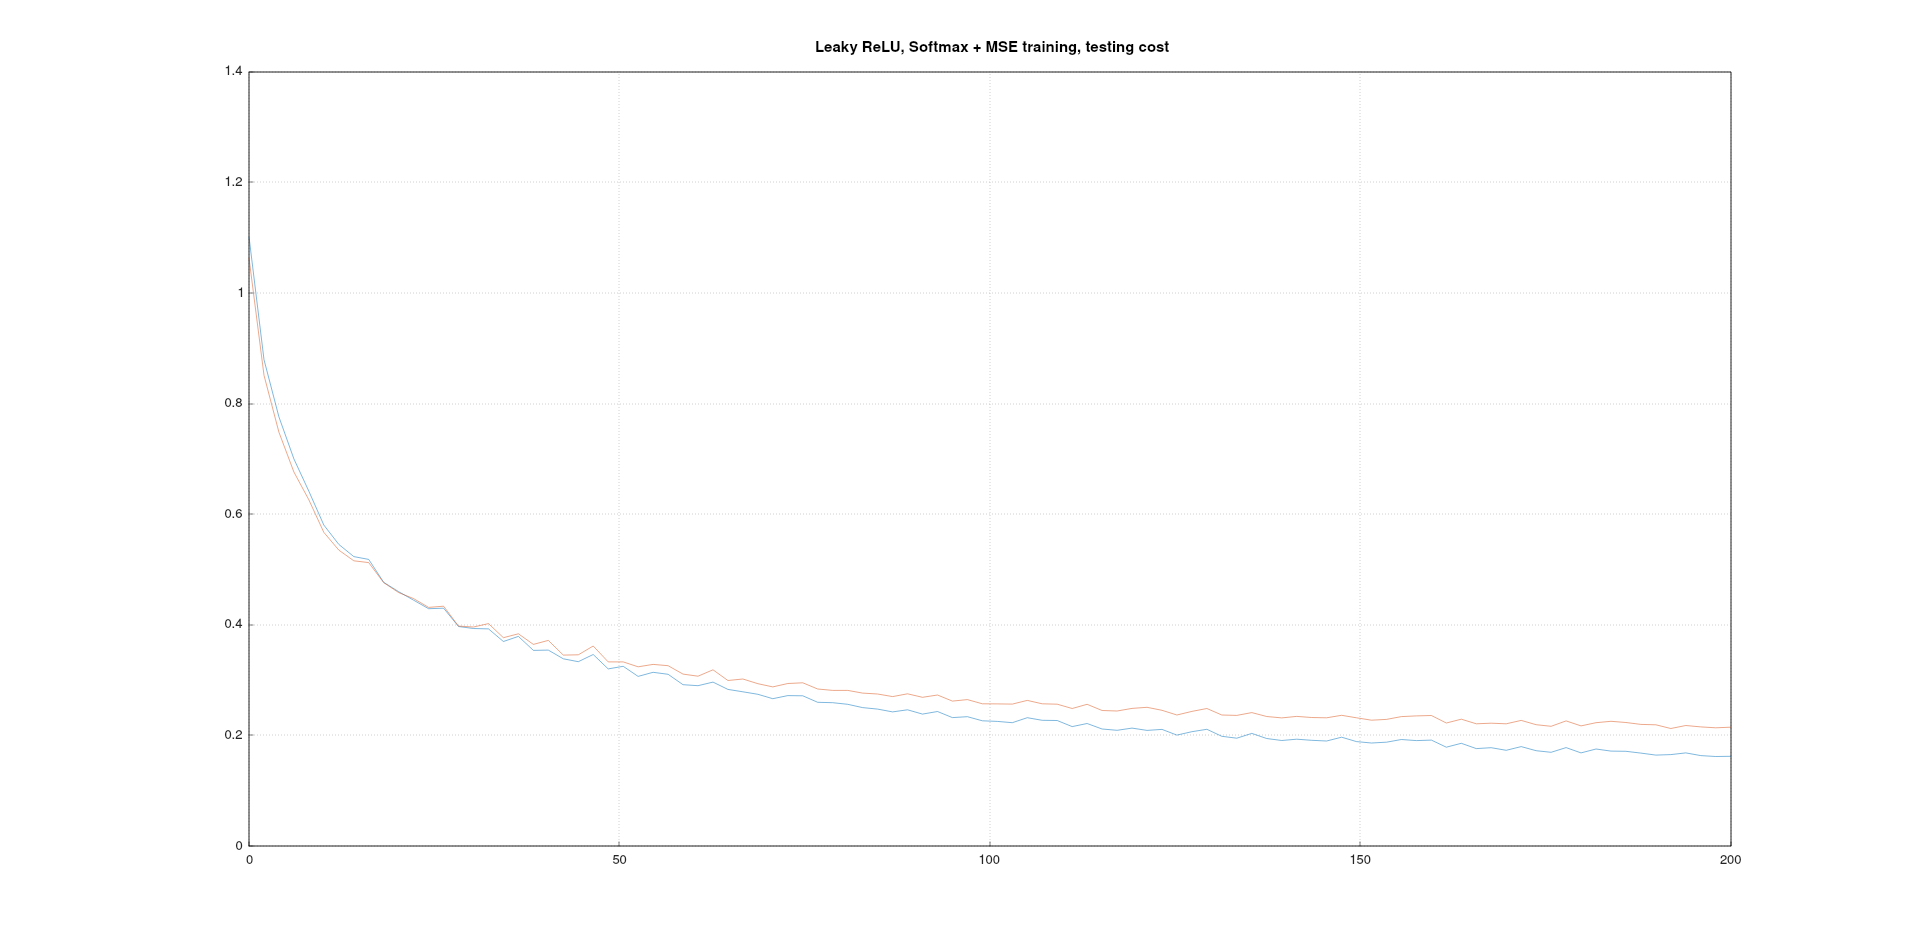
\includegraphics[width=\textwidth]{images/3_40_leaky_relu_softmax_mse_cost.png}
  \caption{}
  \label{fig:3_40_leaky_relu_softmax_mse_cost}
\end{figure}

На рисунке \ref{fig:3_40_leaky_relu_softmax_mse_accuracy} изображено изменение точности за период обучения персептрона.
В результате, точность на данных для обучения составляет $\frac{48422}{50000} \approx 96,84\%$, на тестовых данных --- $\frac{9481}{10000} = 94,81\%$.

\begin{figure}[!htb]
  \centering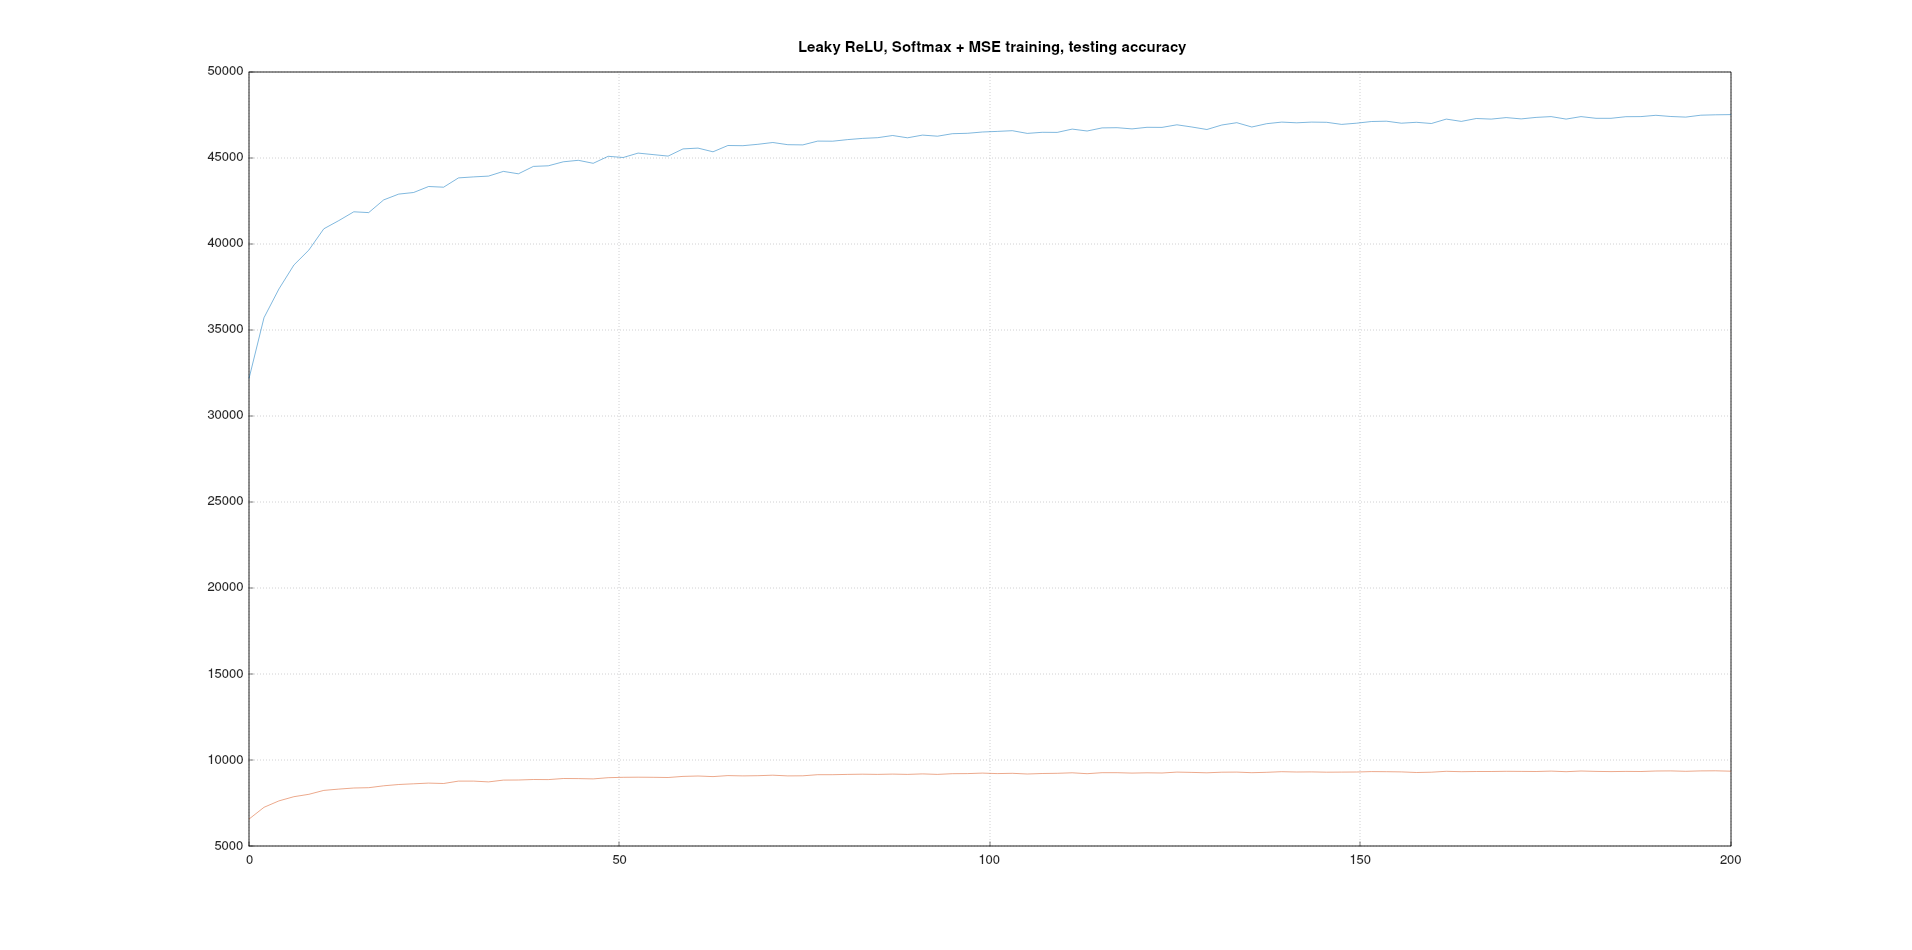
\includegraphics[width=\textwidth]{images/3_40_leaky_relu_softmax_mse_accuracy.png}
  \caption{}
  \label{fig:3_40_leaky_relu_softmax_mse_accuracy}
\end{figure}

\subsection{Перекрёстная энтропия}

\subsubsection{1 скрытый слой, 20 нейронов}

%  Epoch 199; training cost: 0.192402; training accuracy: 47194/50000; testing cost: 0.217352; testing accuracy: 9345/10000;

На рисунке \ref{fig:1_20_leaky_relu_softmax_cross_entropy_cost} изображено изменение функции ошибки за период обучения персептрона.
В результате, ошибка на данных для обучения составляет $0.192402$, ошибка на тестовых данных --- $0.217352$.

\begin{figure}[!htb]
  \centering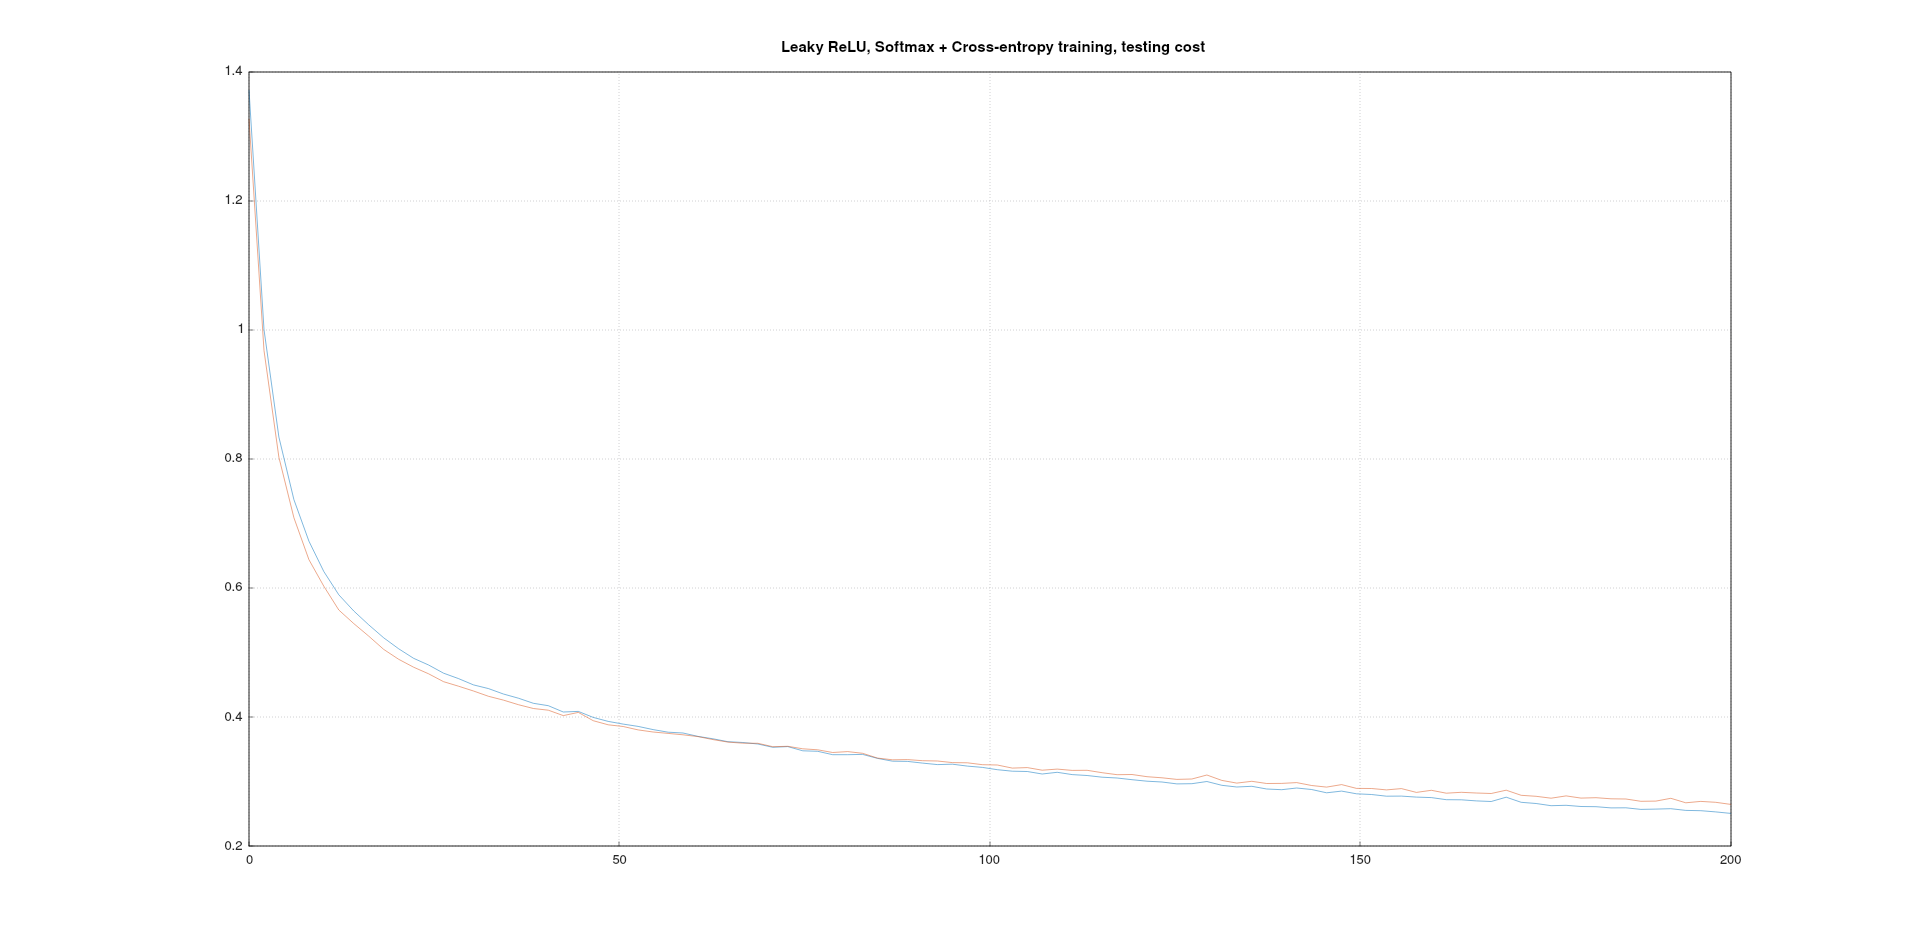
\includegraphics[width=\textwidth]{images/1_20_leaky_relu_softmax_cross_entropy_cost.png}
  \caption{}
  \label{fig:1_20_leaky_relu_softmax_cross_entropy_cost}
\end{figure}

На рисунке \ref{fig:1_20_leaky_relu_softmax_cross_entropy_accuracy} изображено изменение точности за период обучения персептрона.
В результате, точность на данных для обучения составляет $\frac{47194}{50000} \approx 94,34\%$, на тестовых данных --- $\frac{9345}{10000} = 93,45\%$.

\begin{figure}[!htb]
  \centering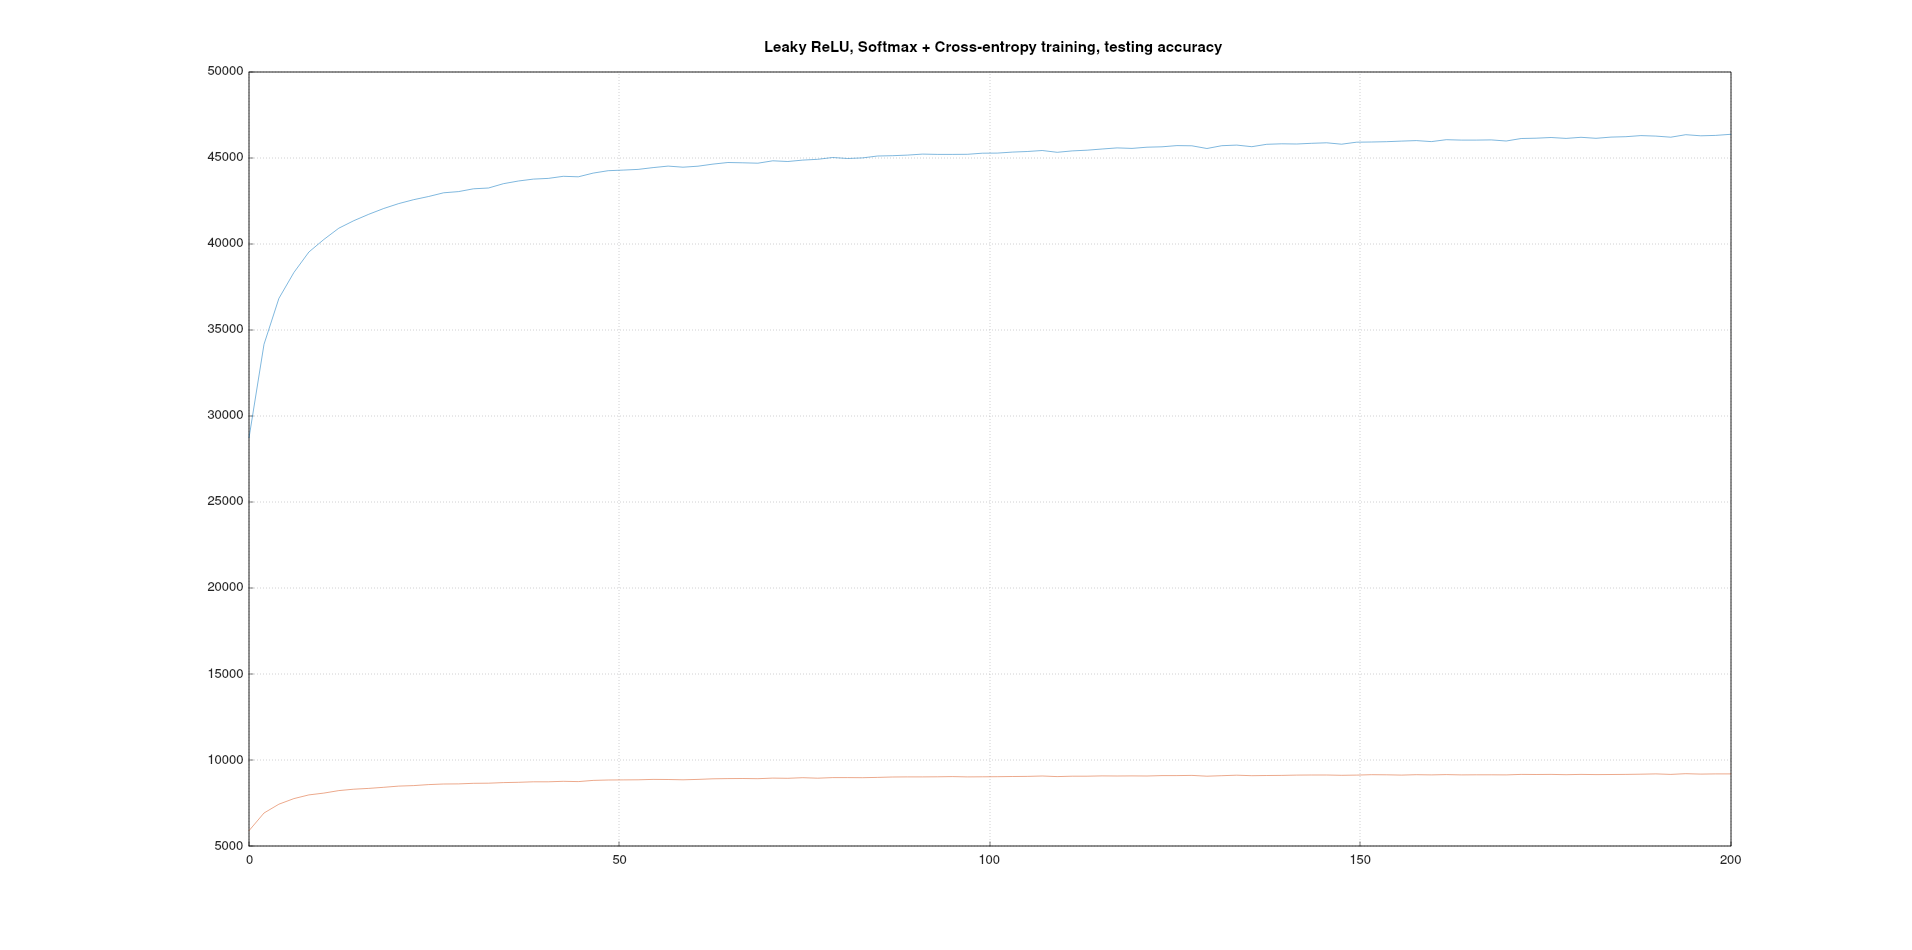
\includegraphics[width=\textwidth]{images/1_20_leaky_relu_softmax_cross_entropy_accuracy.png}
  \caption{}
  \label{fig:1_20_leaky_relu_softmax_cross_entropy_accuracy}
\end{figure}

\subsubsection{1 скрытый слой, 40 нейронов}

%  Epoch 199; training cost: 0.131022; training accuracy: 48097/50000; testing cost: 0.173189; testing accuracy: 9483/10000;

На рисунке \ref{fig:1_40_leaky_relu_softmax_cross_entropy_cost} изображено изменение функции ошибки за период обучения персептрона.
В результате, ошибка на данных для обучения составляет $0.131022$, ошибка на тестовых данных --- $0.173189$.

\begin{figure}[!htb]
  \centering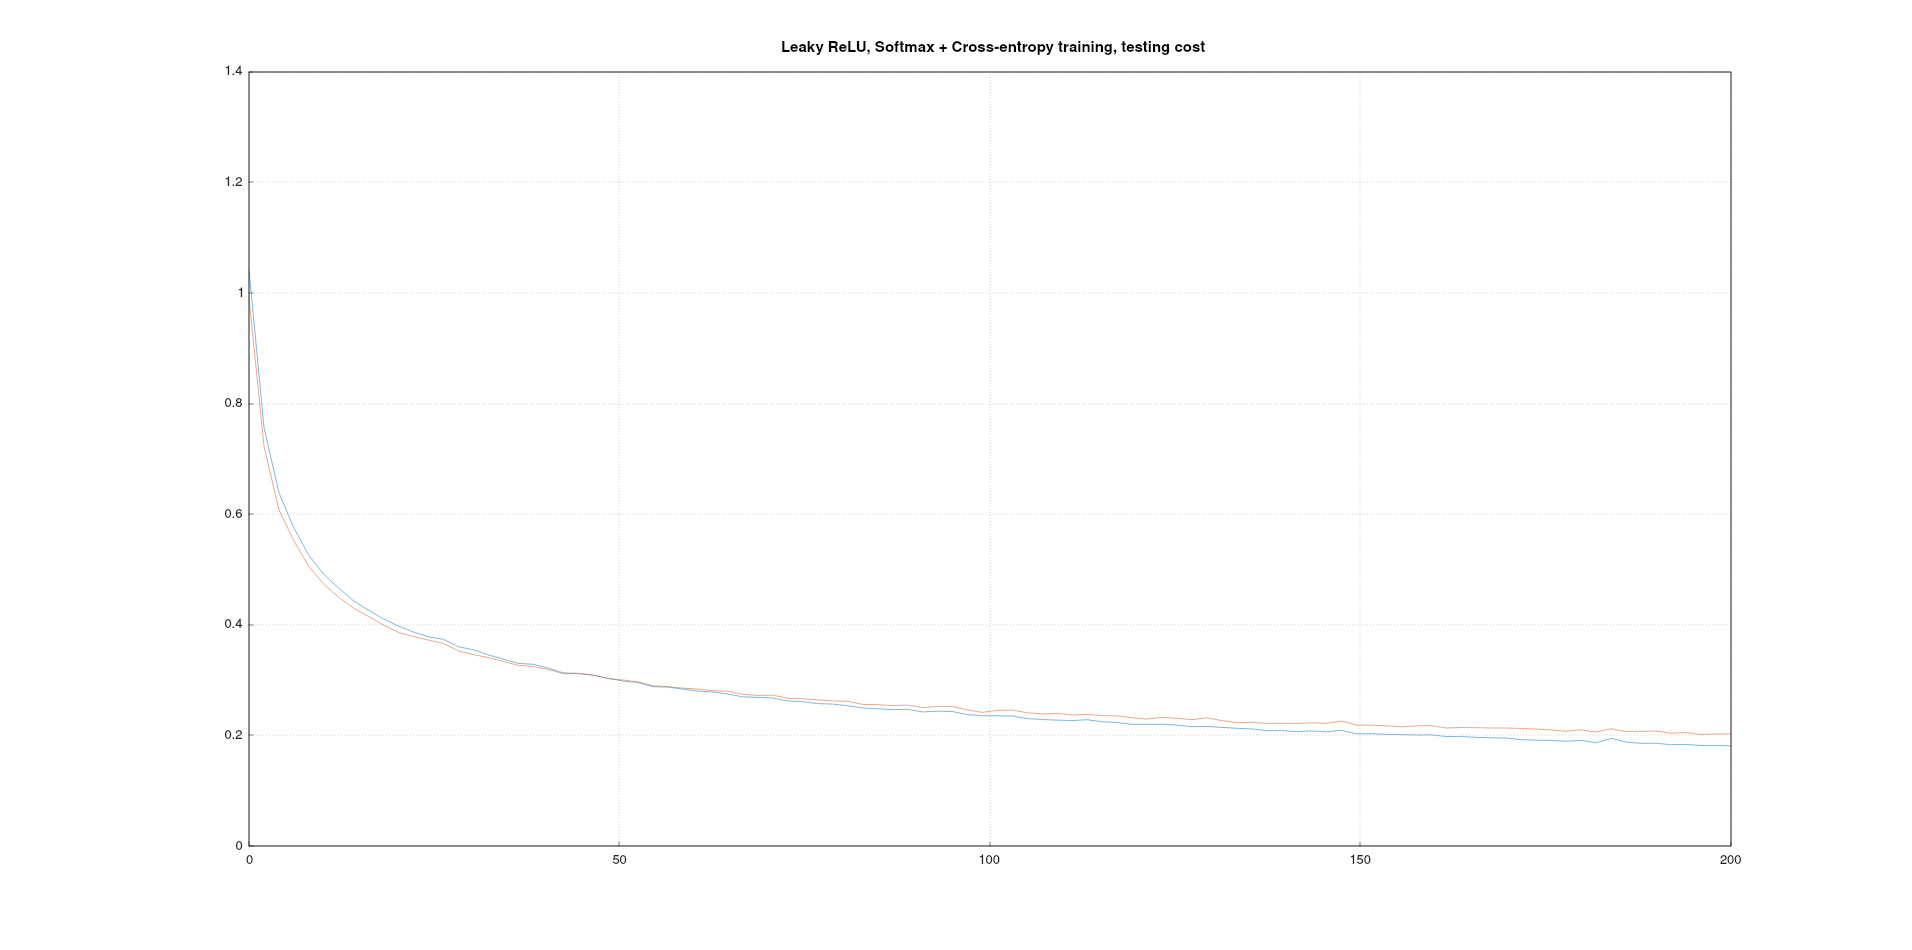
\includegraphics[width=\textwidth]{images/1_40_leaky_relu_softmax_cross_entropy_cost.png}
  \caption{}
  \label{fig:1_40_leaky_relu_softmax_cross_entropy_cost}
\end{figure}

На рисунке \ref{fig:1_40_leaky_relu_softmax_cross_entropy_accuracy} изображено изменение точности за период обучения персептрона.
В результате, точность на данных для обучения составляет $\frac{48097}{50000} \approx 96,19\%$, на тестовых данных --- $\frac{9483}{10000} = 94,83\%$.

\begin{figure}[!htb]
  \centering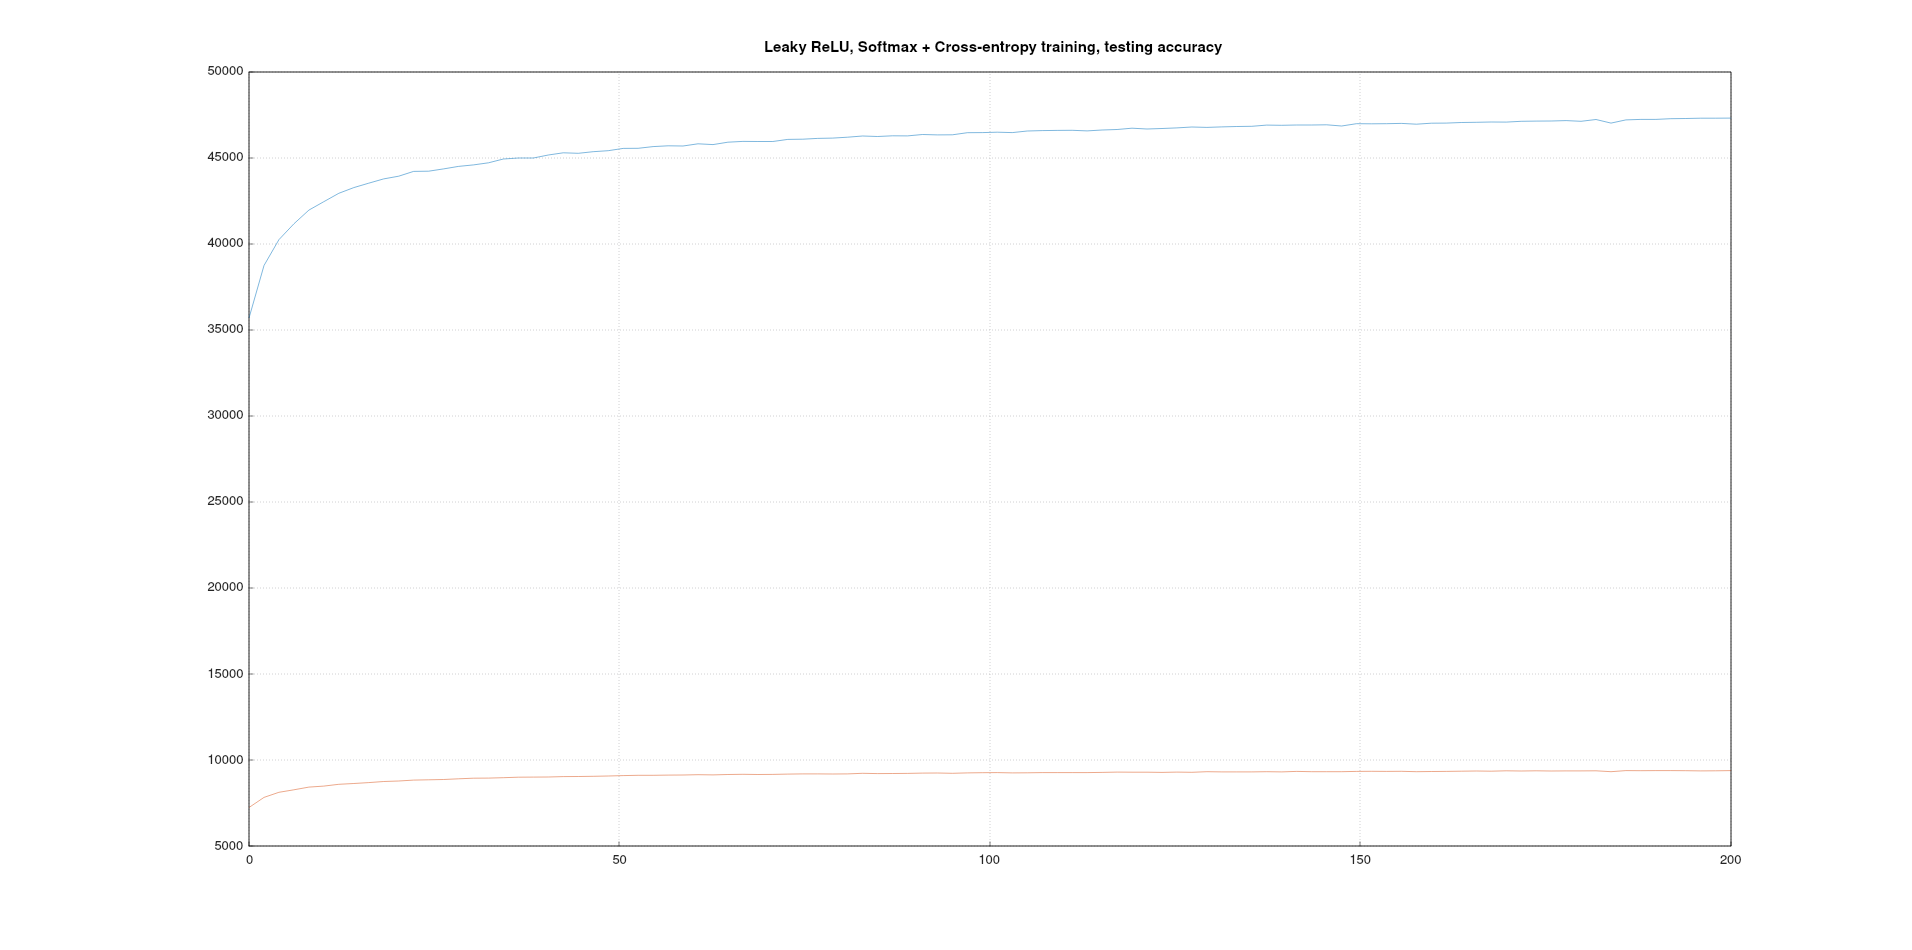
\includegraphics[width=\textwidth]{images/1_40_leaky_relu_softmax_cross_entropy_accuracy.png}
  \caption{}
  \label{fig:1_40_leaky_relu_softmax_cross_entropy_accuracy}
\end{figure}

\subsubsection{3 скрытых слоя, 20 нейронов}

%  Epoch 199; training cost: 0.157613; training accuracy: 47681/50000; testing cost: 0.216353; testing accuracy: 9386/10000;

На рисунке \ref{fig:3_20_leaky_relu_softmax_cross_entropy_cost} изображено изменение функции ошибки за период обучения персептрона.
В результате, ошибка на данных для обучения составляет $0.157613$, ошибка на тестовых данных --- $0.216353$.

\begin{figure}[!htb]
  \centering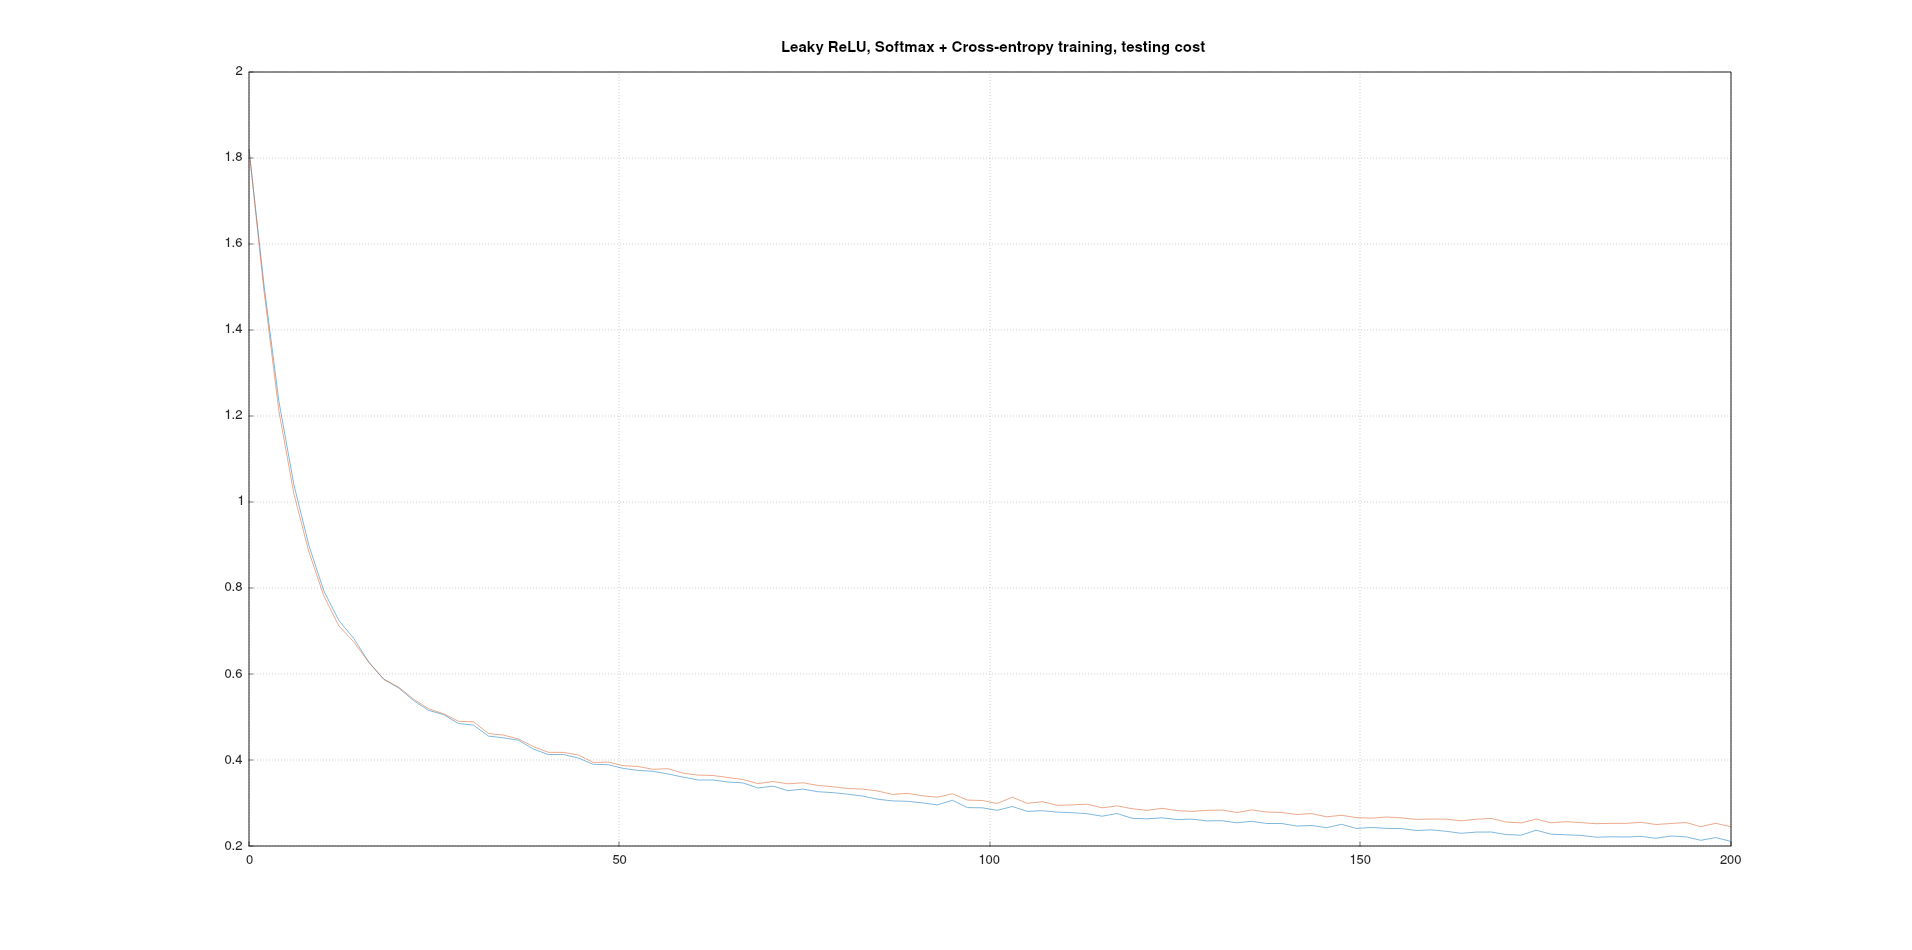
\includegraphics[width=\textwidth]{images/3_20_leaky_relu_softmax_cross_entropy_cost.png}
  \caption{}
  \label{fig:3_20_leaky_relu_softmax_cross_entropy_cost}
\end{figure}

На рисунке \ref{fig:3_20_leaky_relu_softmax_cross_entropy_accuracy} изображено изменение точности за период обучения персептрона.
В результате, точность на данных для обучения составляет $\frac{47681}{50000} \approx 95,36\%$, на тестовых данных --- $\frac{9386}{10000} = 93,86\%$.

\begin{figure}[!htb]
  \centering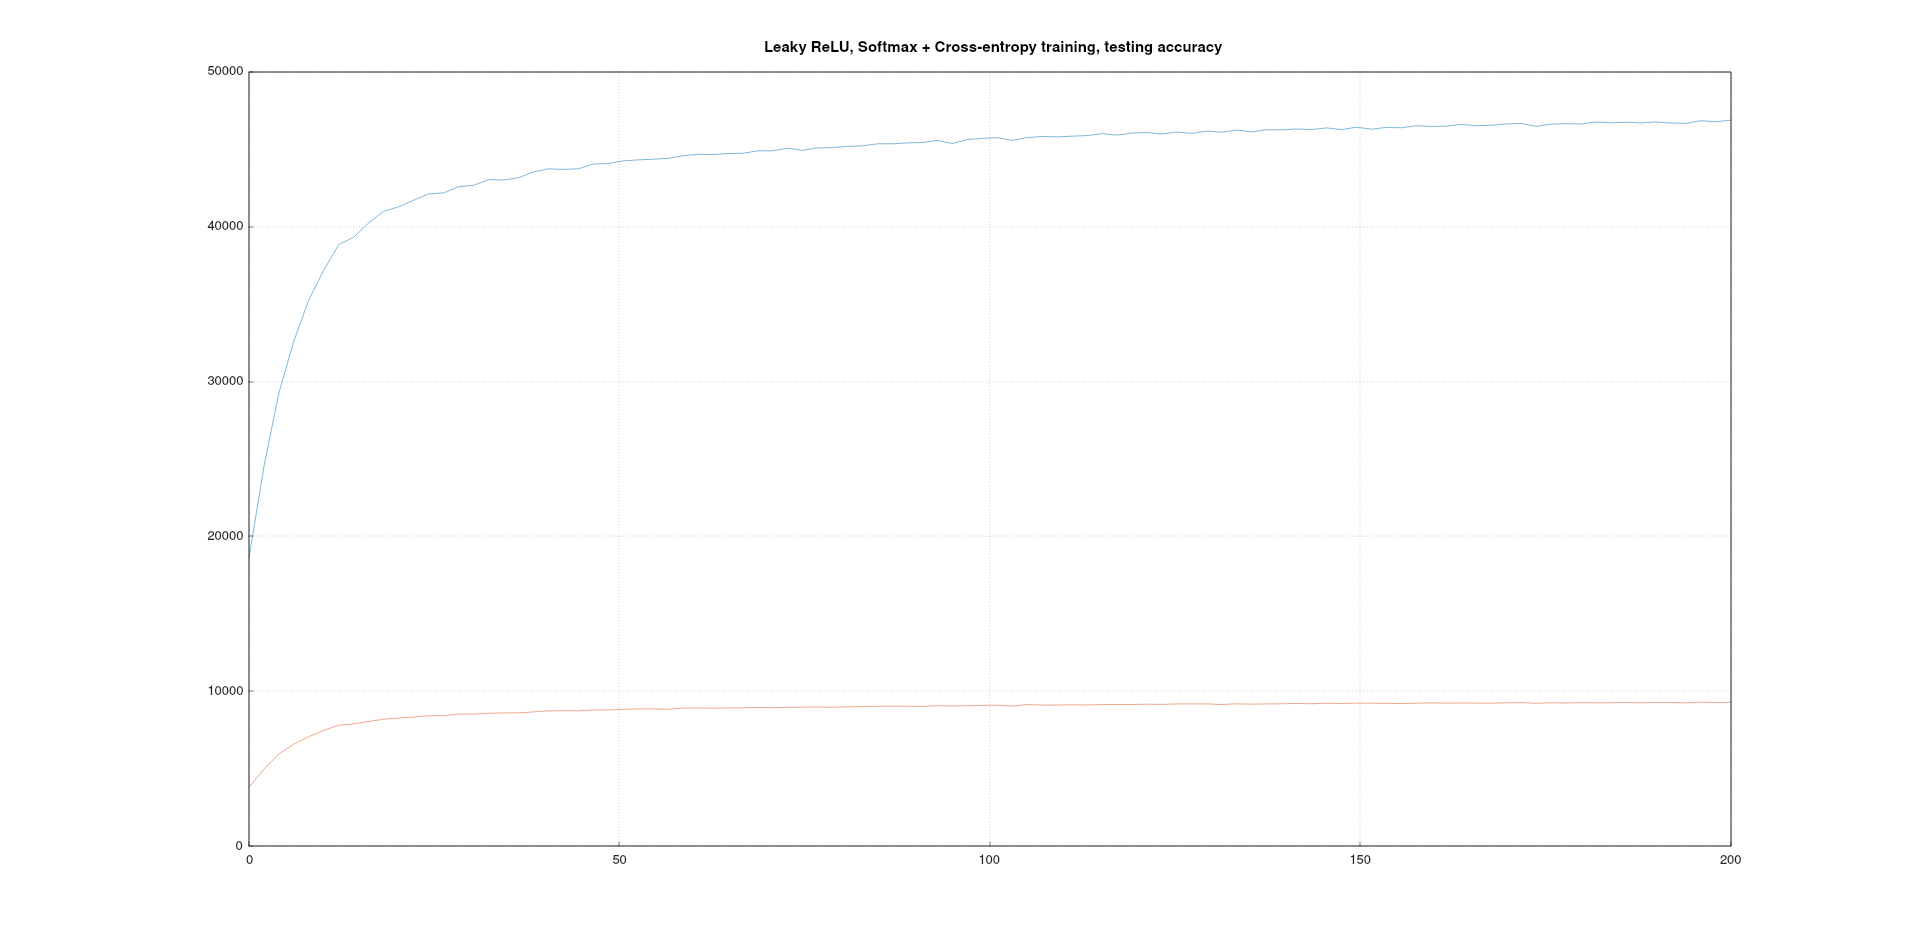
\includegraphics[width=\textwidth]{images/3_20_leaky_relu_softmax_cross_entropy_accuracy.png}
  \caption{}
  \label{fig:3_20_leaky_relu_softmax_cross_entropy_accuracy}
\end{figure}

\subsubsection{3 скрытых слоя, 40 нейронов}

%  Epoch 199; training cost: 0.118457; training accuracy: 48232/50000; testing cost: 0.17582; testing accuracy: 9502/10000;

На рисунке \ref{fig:3_40_leaky_relu_softmax_cross_entropy_cost} изображено изменение функции ошибки за период обучения персептрона.
В результате, ошибка на данных для обучения составляет $0.118457$, ошибка на тестовых данных --- $0.17582$.

\begin{figure}[!htb]
  \centering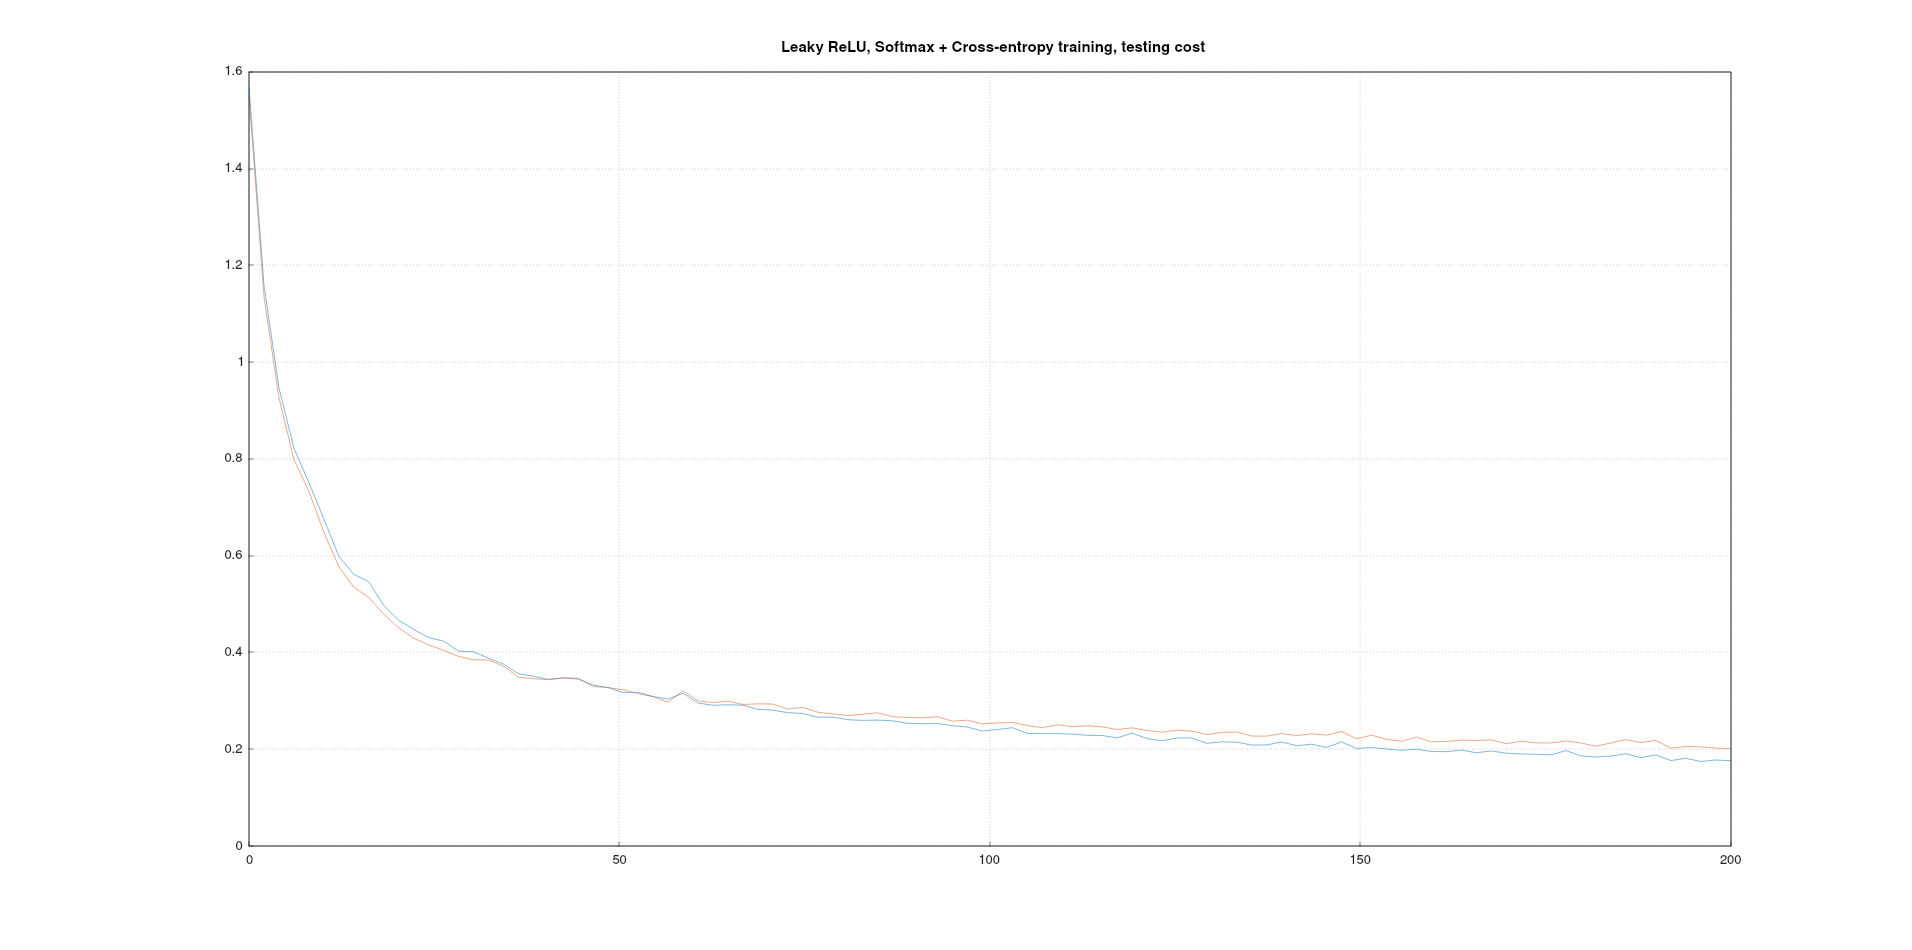
\includegraphics[width=\textwidth]{images/3_40_leaky_relu_softmax_cross_entropy_cost.png}
  \caption{}
  \label{fig:3_40_leaky_relu_softmax_cross_entropy_cost}
\end{figure}

На рисунке \ref{fig:3_40_leaky_relu_softmax_cross_entropy_accuracy} изображено изменение точности за период обучения персептрона.
В результате, точность на данных для обучения составляет $\frac{48232}{50000} \approx 96,46\%$, на тестовых данных --- $\frac{9502}{10000} = 95,02\%$.

\begin{figure}[!htb]
  \centering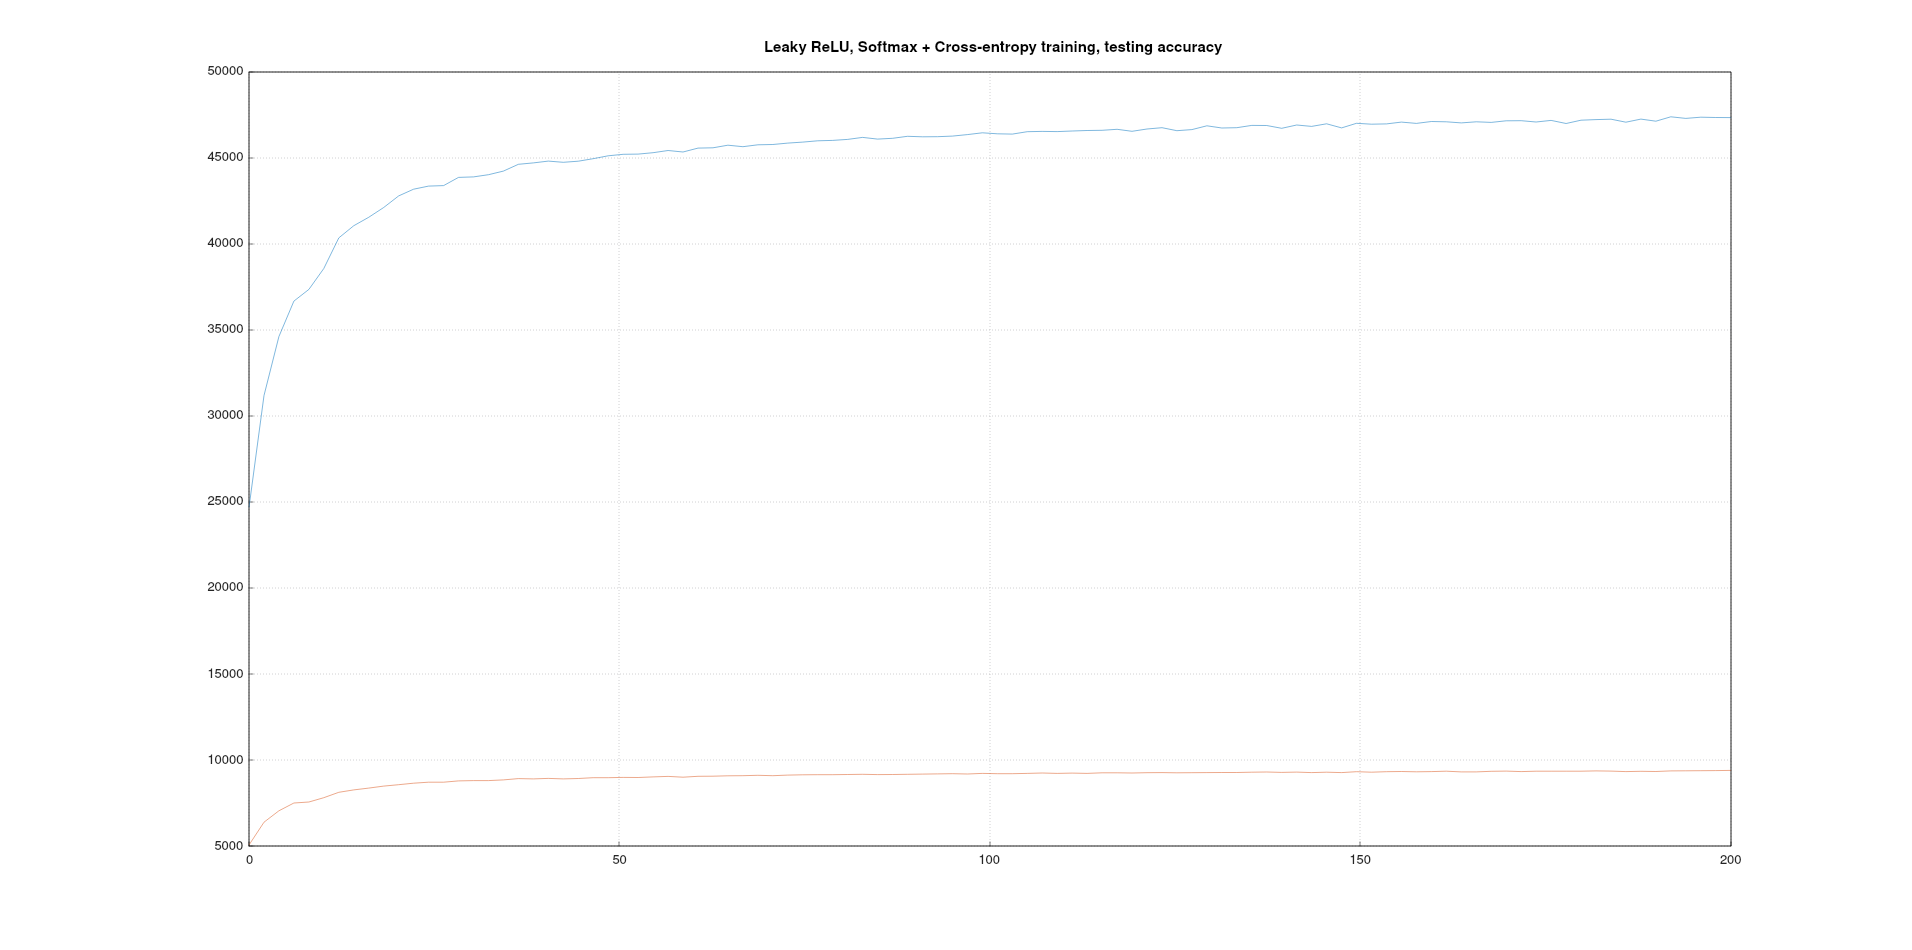
\includegraphics[width=\textwidth]{images/3_40_leaky_relu_softmax_cross_entropy_accuracy.png}
  \caption{}
  \label{fig:3_40_leaky_relu_softmax_cross_entropy_accuracy}
\end{figure}

\subsection{Дивергенция Кульбака-Лейблера}

\subsubsection{1 скрытый слой, 20 нейронов}

%  Epoch 199; training cost: 0.17601; training accuracy: 47346/50000; testing cost: 0.201559; testing accuracy: 9415/10000;

На рисунке \ref{fig:1_20_leaky_relu_softmax_kl_divergence_cost} изображено изменение функции ошибки за период обучения персептрона.
В результате, ошибка на данных для обучения составляет $0.17601$, ошибка на тестовых данных --- $0.201559$.

\begin{figure}[!htb]
  \centering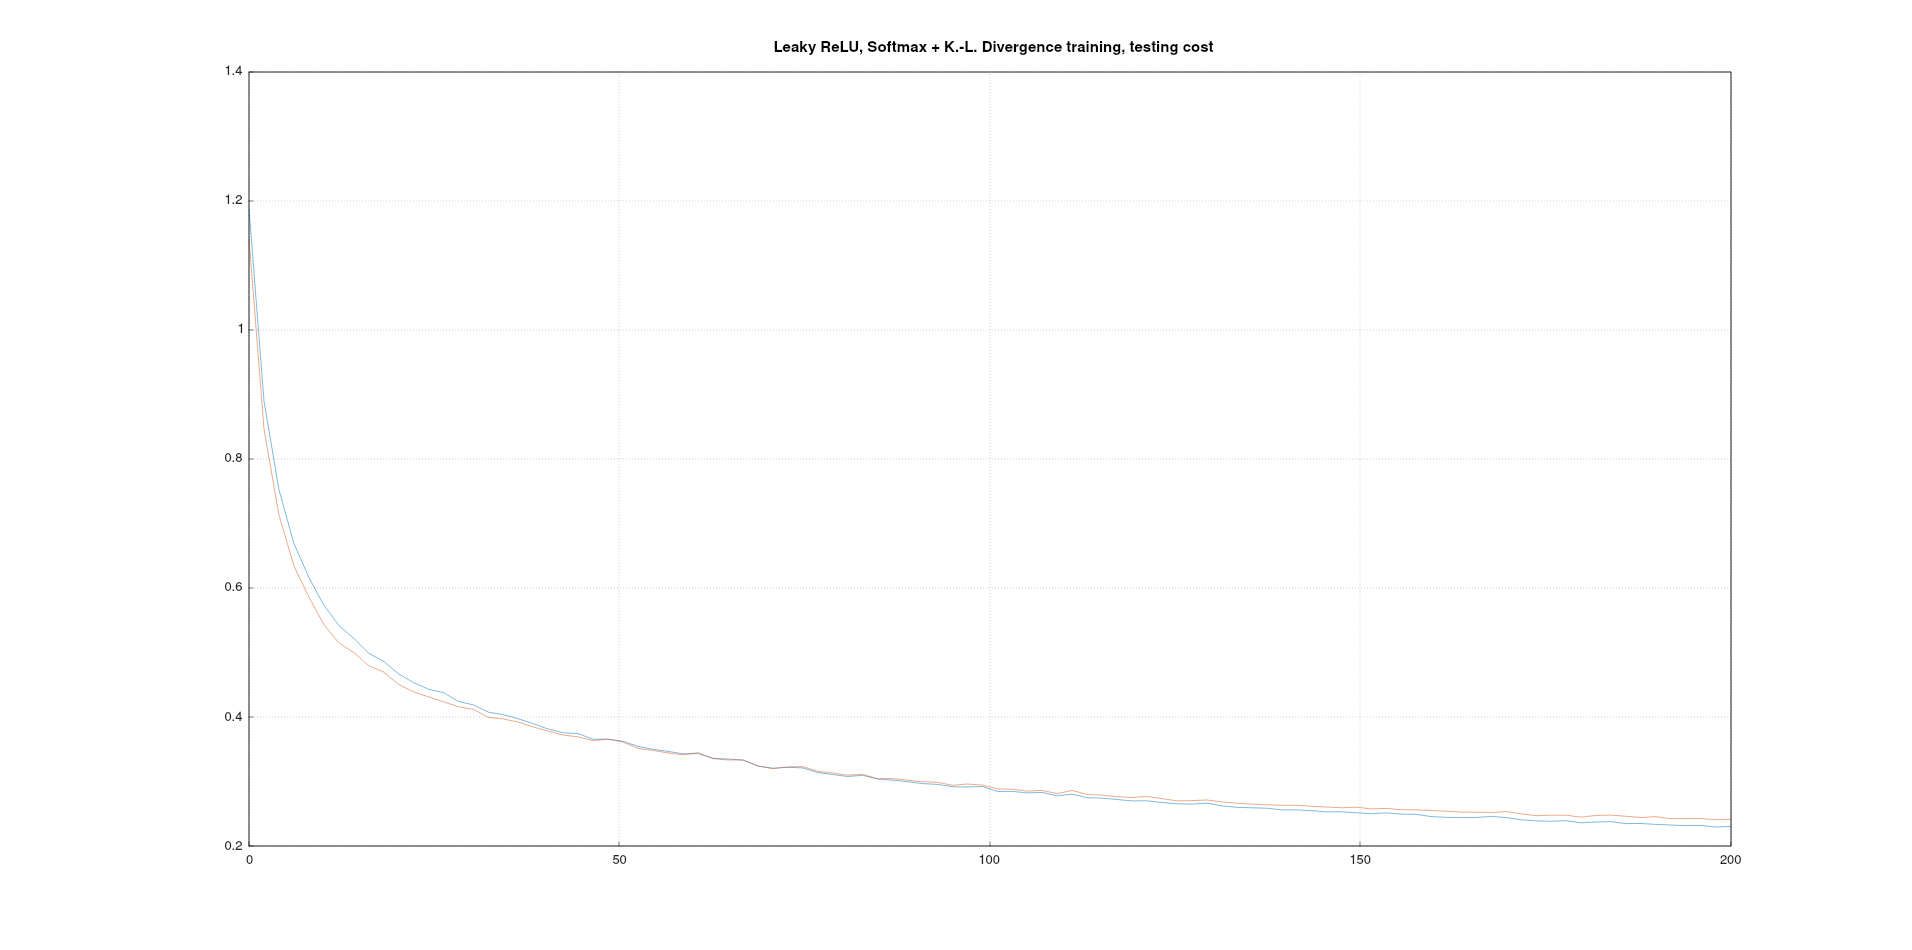
\includegraphics[width=\textwidth]{images/1_20_leaky_relu_softmax_kl_divergence_cost.png}
  \caption{}
  \label{fig:1_20_leaky_relu_softmax_kl_divergence_cost}
\end{figure}

На рисунке \ref{fig:1_20_leaky_relu_softmax_kl_divergence_accuracy} изображено изменение точности за период обучения персептрона.
В результате, точность на данных для обучения составляет $\frac{47346}{50000} \approx 94,69\%$, на тестовых данных --- $\frac{9415}{10000} = 94,15\%$.

\begin{figure}[!htb]
  \centering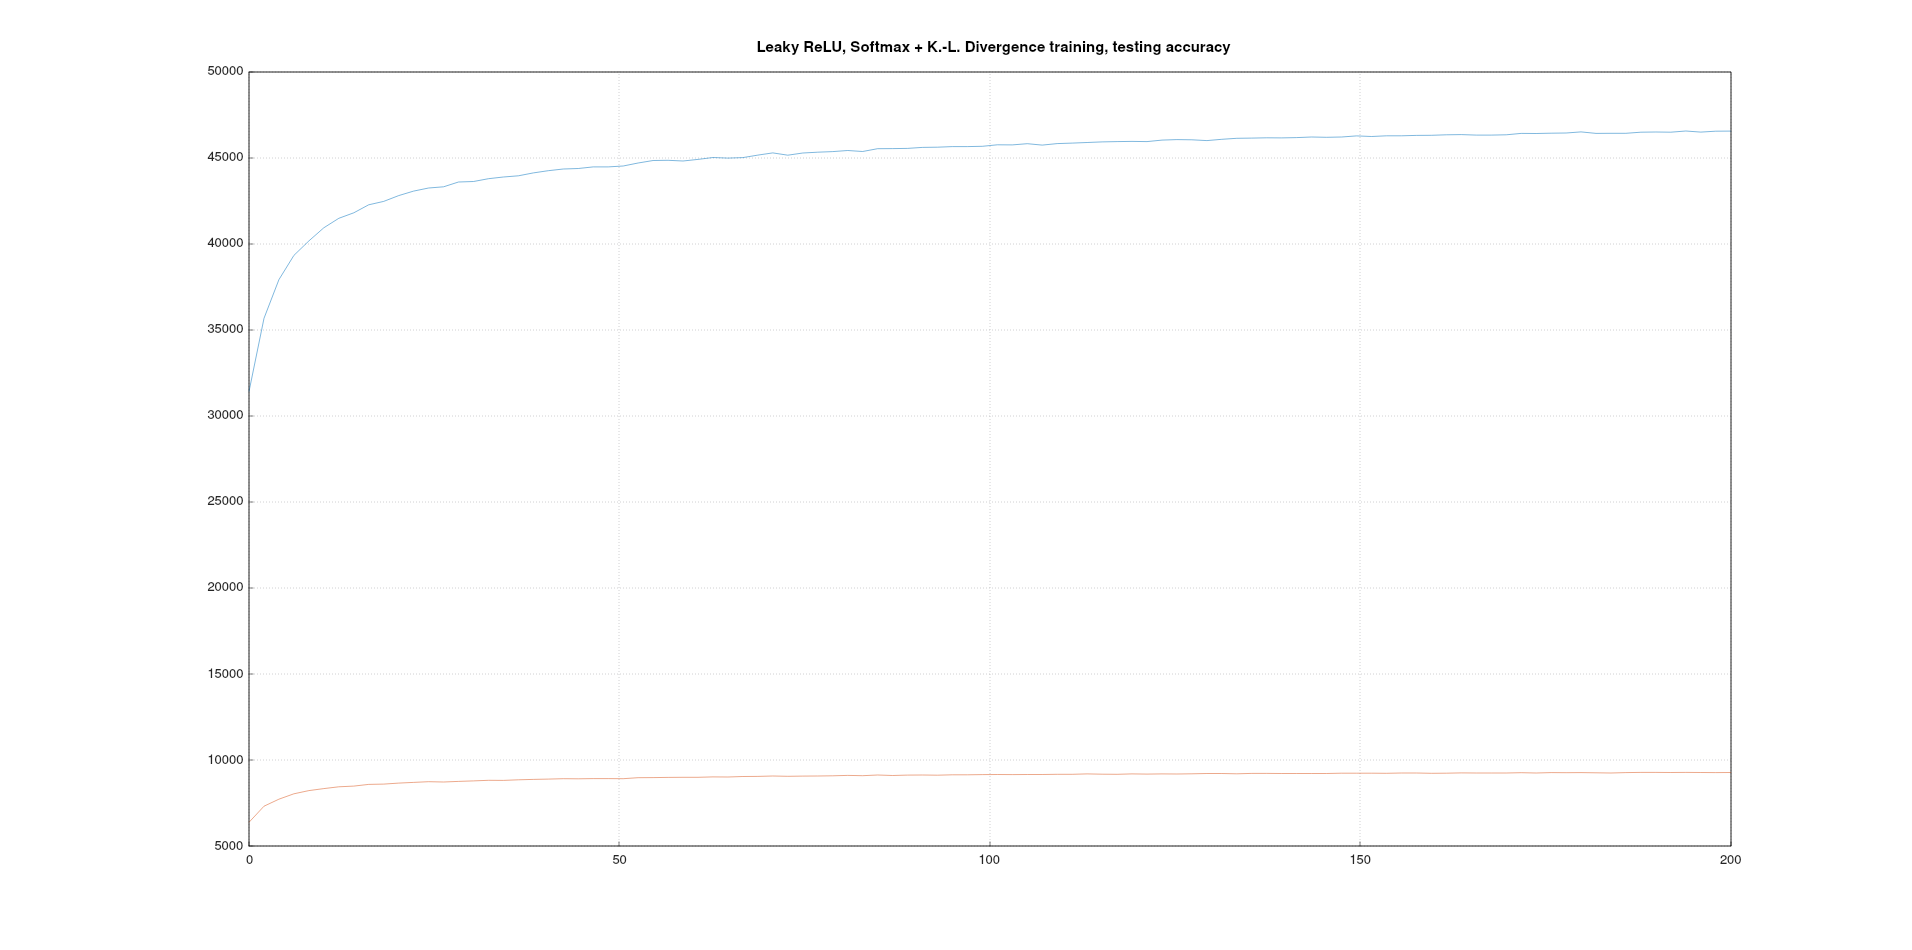
\includegraphics[width=\textwidth]{images/1_20_leaky_relu_softmax_kl_divergence_accuracy.png}
  \caption{}
  \label{fig:1_20_leaky_relu_softmax_kl_divergence_accuracy}
\end{figure}

\subsubsection{1 скрытый слой, 40 нейронов}

%  Epoch 199; training cost: 0.118821; training accuracy: 48233/50000; testing cost: 0.168346; testing accuracy: 9506/10000;

На рисунке \ref{fig:1_40_leaky_relu_softmax_kl_divergence_cost} изображено изменение функции ошибки за период обучения персептрона.
В результате, ошибка на данных для обучения составляет $0.118821$, ошибка на тестовых данных --- $0.168346$.

\begin{figure}[!htb]
  \centering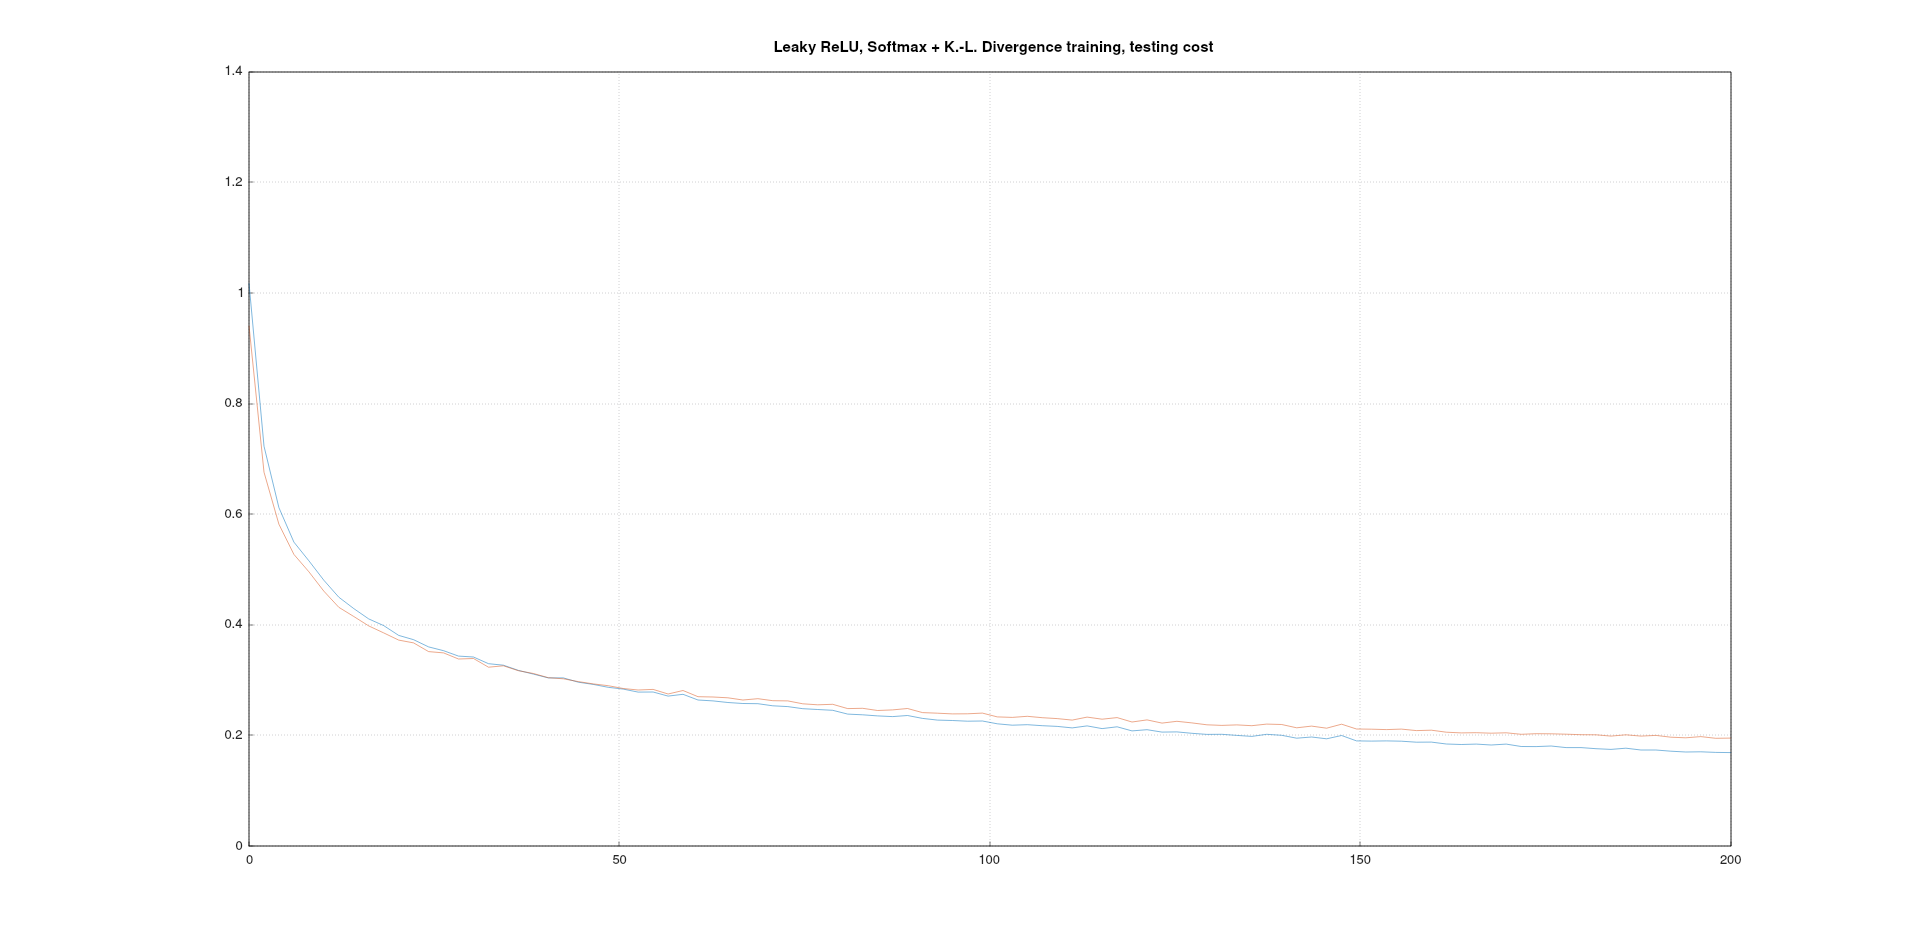
\includegraphics[width=\textwidth]{images/1_40_leaky_relu_softmax_kl_divergence_cost.png}
  \caption{}
  \label{fig:1_40_leaky_relu_softmax_kl_divergence_cost}
\end{figure}

На рисунке \ref{fig:1_40_leaky_relu_softmax_kl_divergence_accuracy} изображено изменение точности за период обучения персептрона.
В результате, точность на данных для обучения составляет $\frac{48233}{50000} \approx 96,47\%$, на тестовых данных --- $\frac{9506}{10000} = 95,06\%$.

\begin{figure}[!htb]
  \centering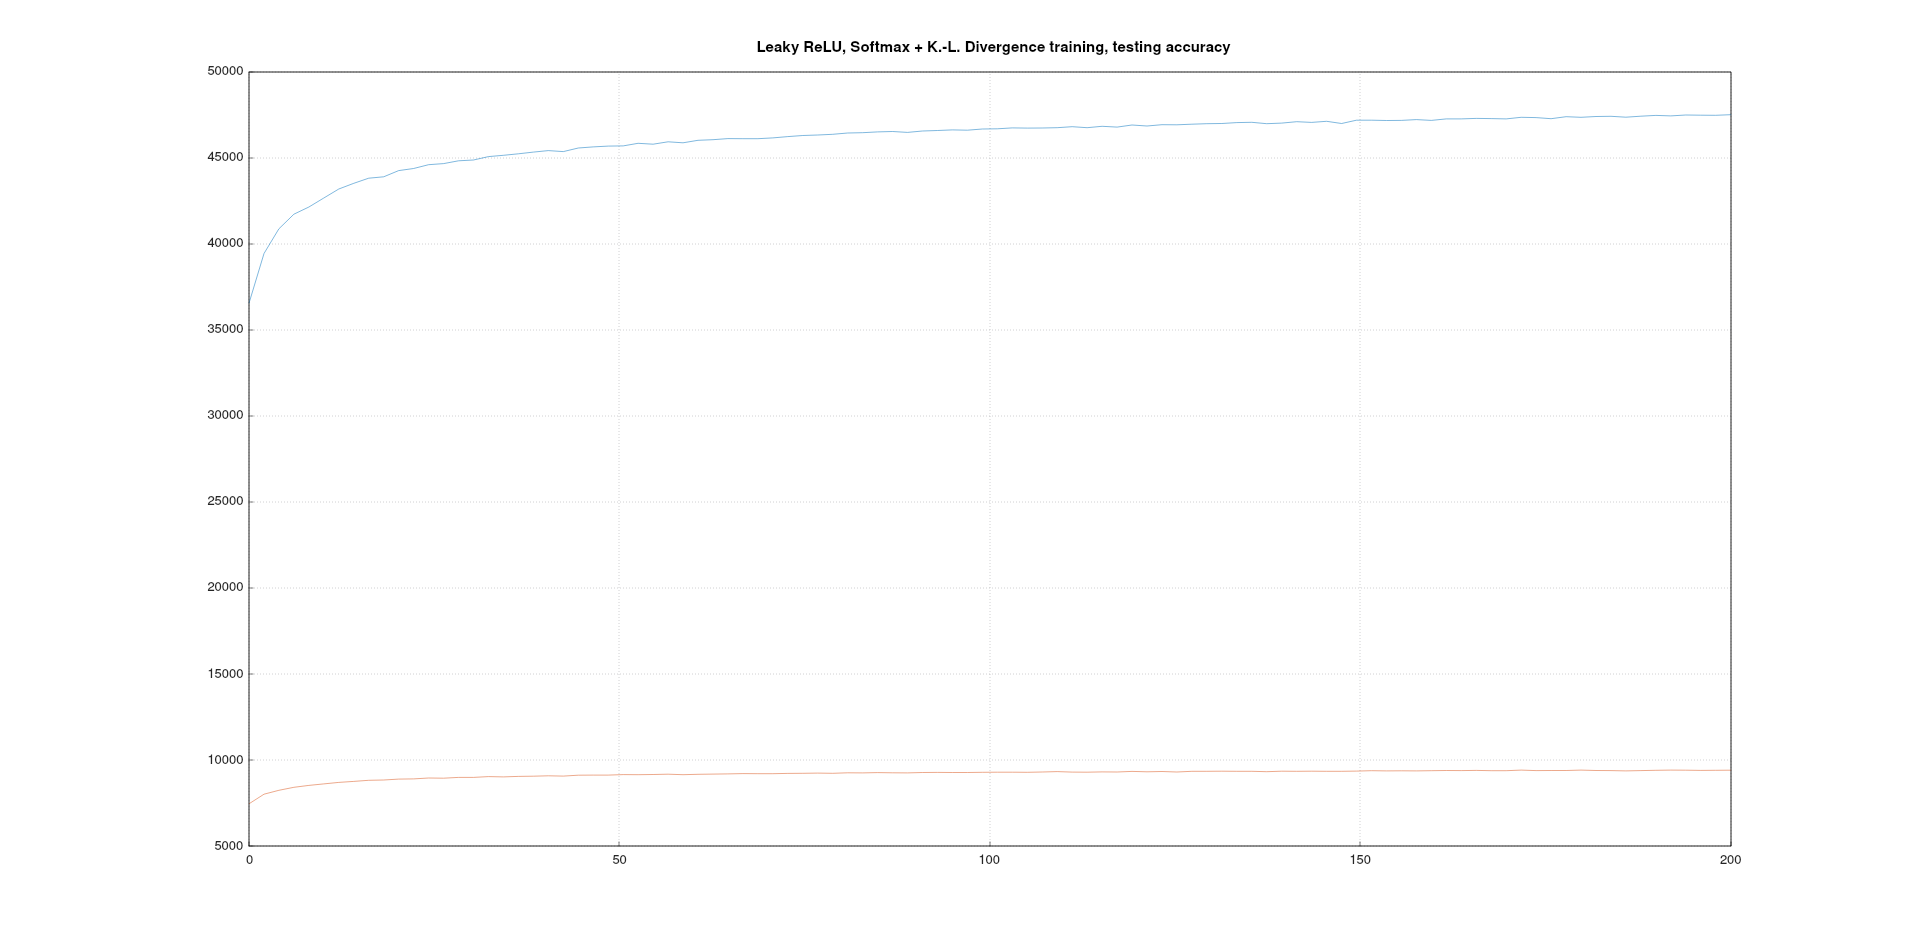
\includegraphics[width=\textwidth]{images/1_40_leaky_relu_softmax_kl_divergence_accuracy.png}
  \caption{}
  \label{fig:1_40_leaky_relu_softmax_kl_divergence_accuracy}
\end{figure}

\subsubsection{3 скрытых слоя, 20 нейронов}

%  Epoch 199; training cost: 0.163792; training accuracy: 47487/50000; testing cost: 0.213412; testing accuracy: 9369/10000;

На рисунке \ref{fig:3_20_leaky_relu_softmax_kl_divergence_cost} изображено изменение функции ошибки за период обучения персептрона.
В результате, ошибка на данных для обучения составляет $0.163792$, ошибка на тестовых данных --- $0.213412$.

\begin{figure}[!htb]
  \centering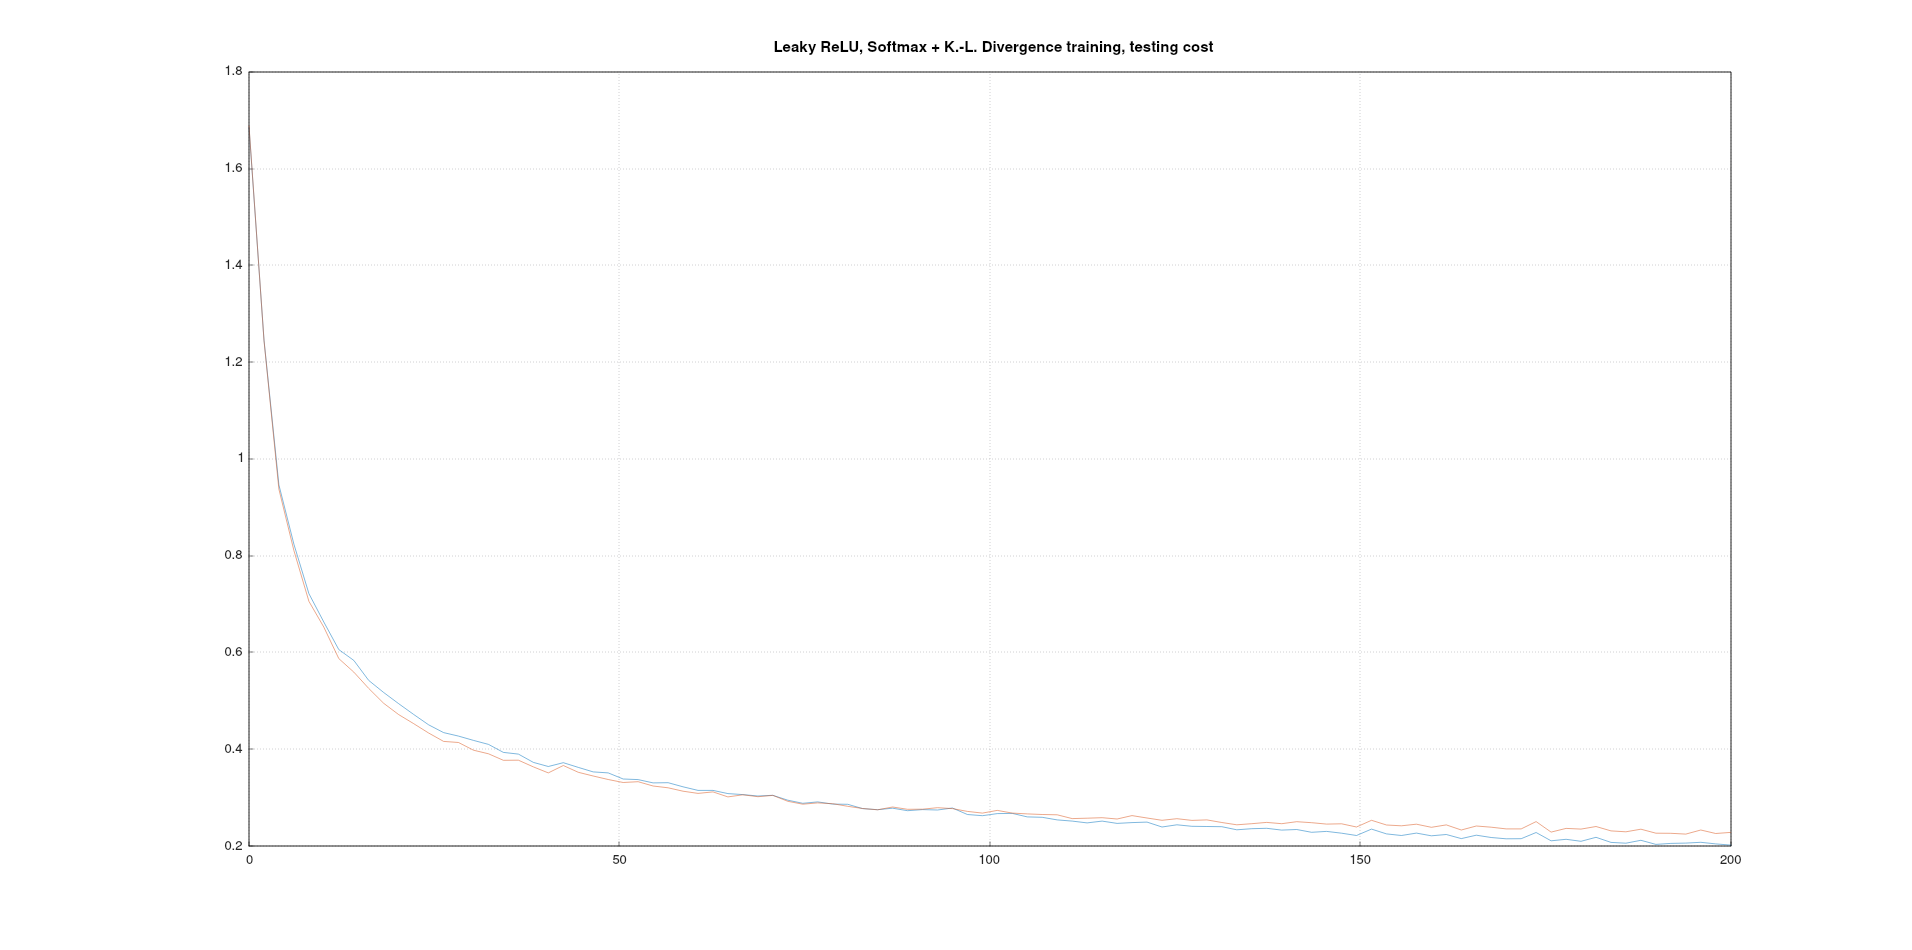
\includegraphics[width=\textwidth]{images/3_20_leaky_relu_softmax_kl_divergence_cost.png}
  \caption{}
  \label{fig:3_20_leaky_relu_softmax_kl_divergence_cost}
\end{figure}

На рисунке \ref{fig:3_20_leaky_relu_softmax_kl_divergence_accuracy} изображено изменение точности за период обучения персептрона.
В результате, точность на данных для обучения составляет $\frac{47487}{50000} \approx 94,97\%$, на тестовых данных --- $\frac{9369}{10000} = 93,69\%$.

\begin{figure}[!htb]
  \centering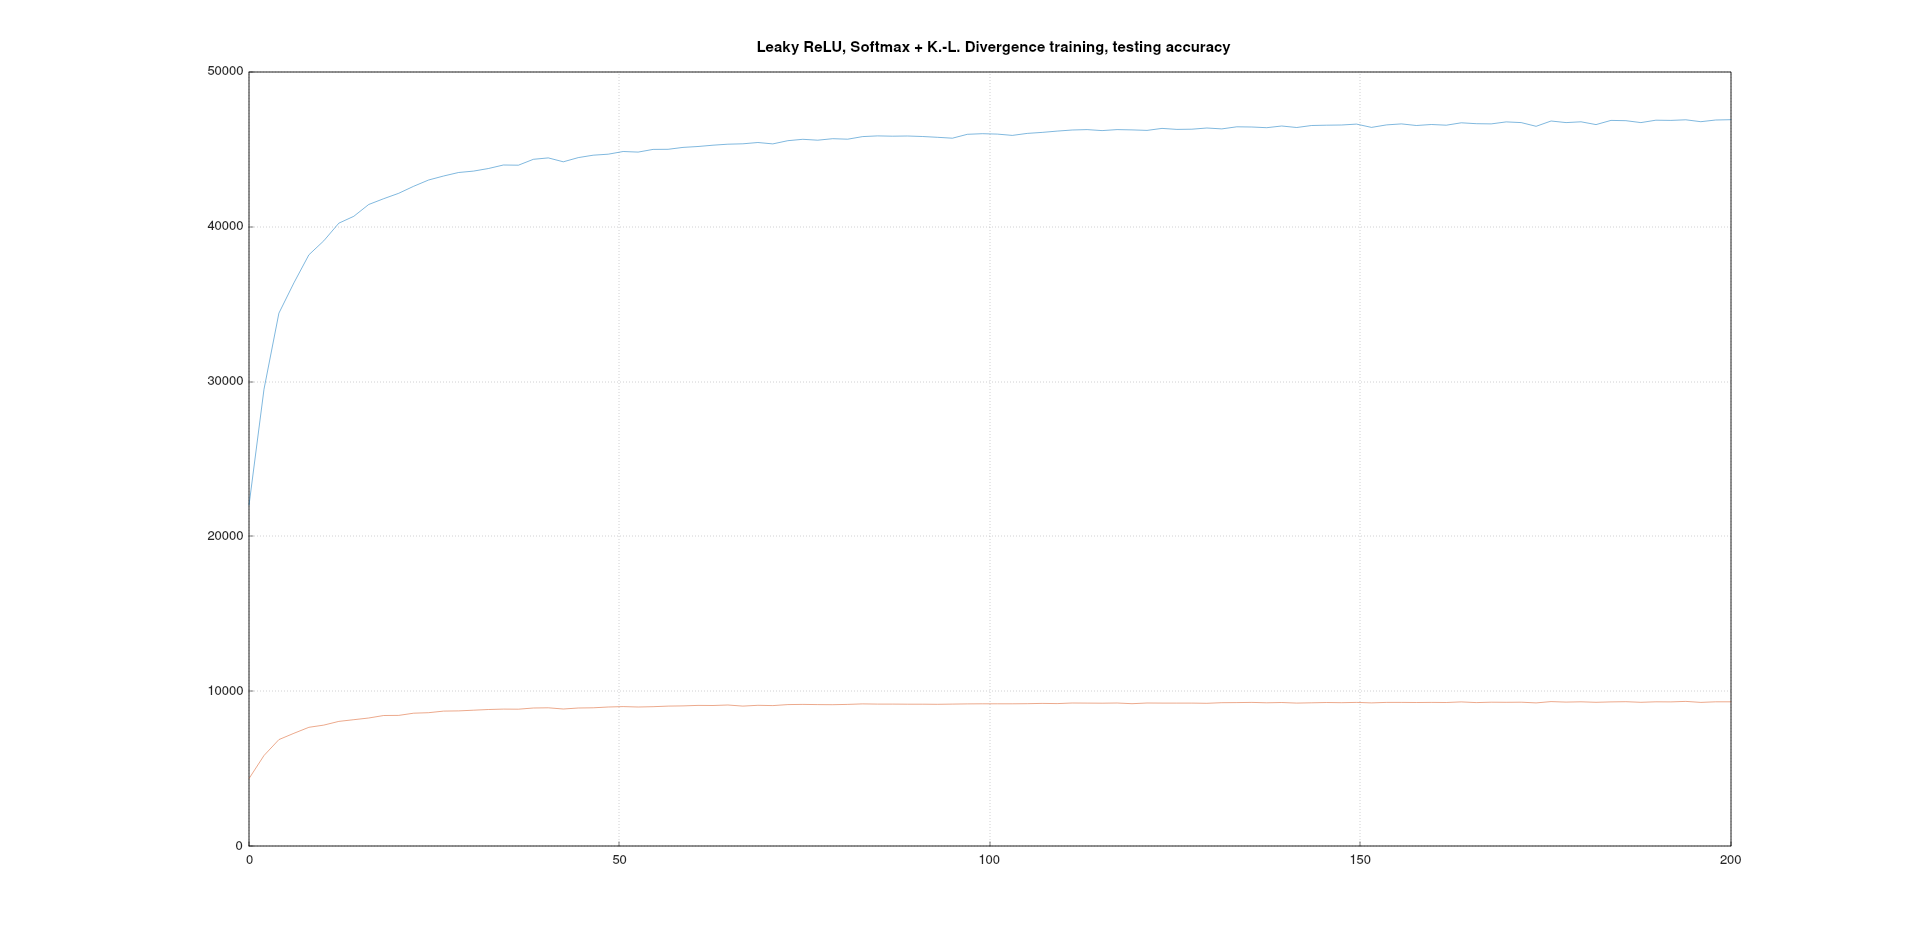
\includegraphics[width=\textwidth]{images/3_20_leaky_relu_softmax_kl_divergence_accuracy.png}
  \caption{}
  \label{fig:3_20_leaky_relu_softmax_kl_divergence_accuracy}
\end{figure}

\subsubsection{3 скрытых слоя, 40 нейронов}

%  Epoch 199; training cost: 0.111865; training accuracy: 48315/50000; testing cost: 0.197848; testing accuracy: 9457/10000;

На рисунке \ref{fig:3_40_leaky_relu_softmax_kl_divergence_cost} изображено изменение функции ошибки за период обучения персептрона.
В результате, ошибка на данных для обучения составляет $0.111865$, ошибка на тестовых данных --- $0.197848$.

\begin{figure}[!htb]
  \centering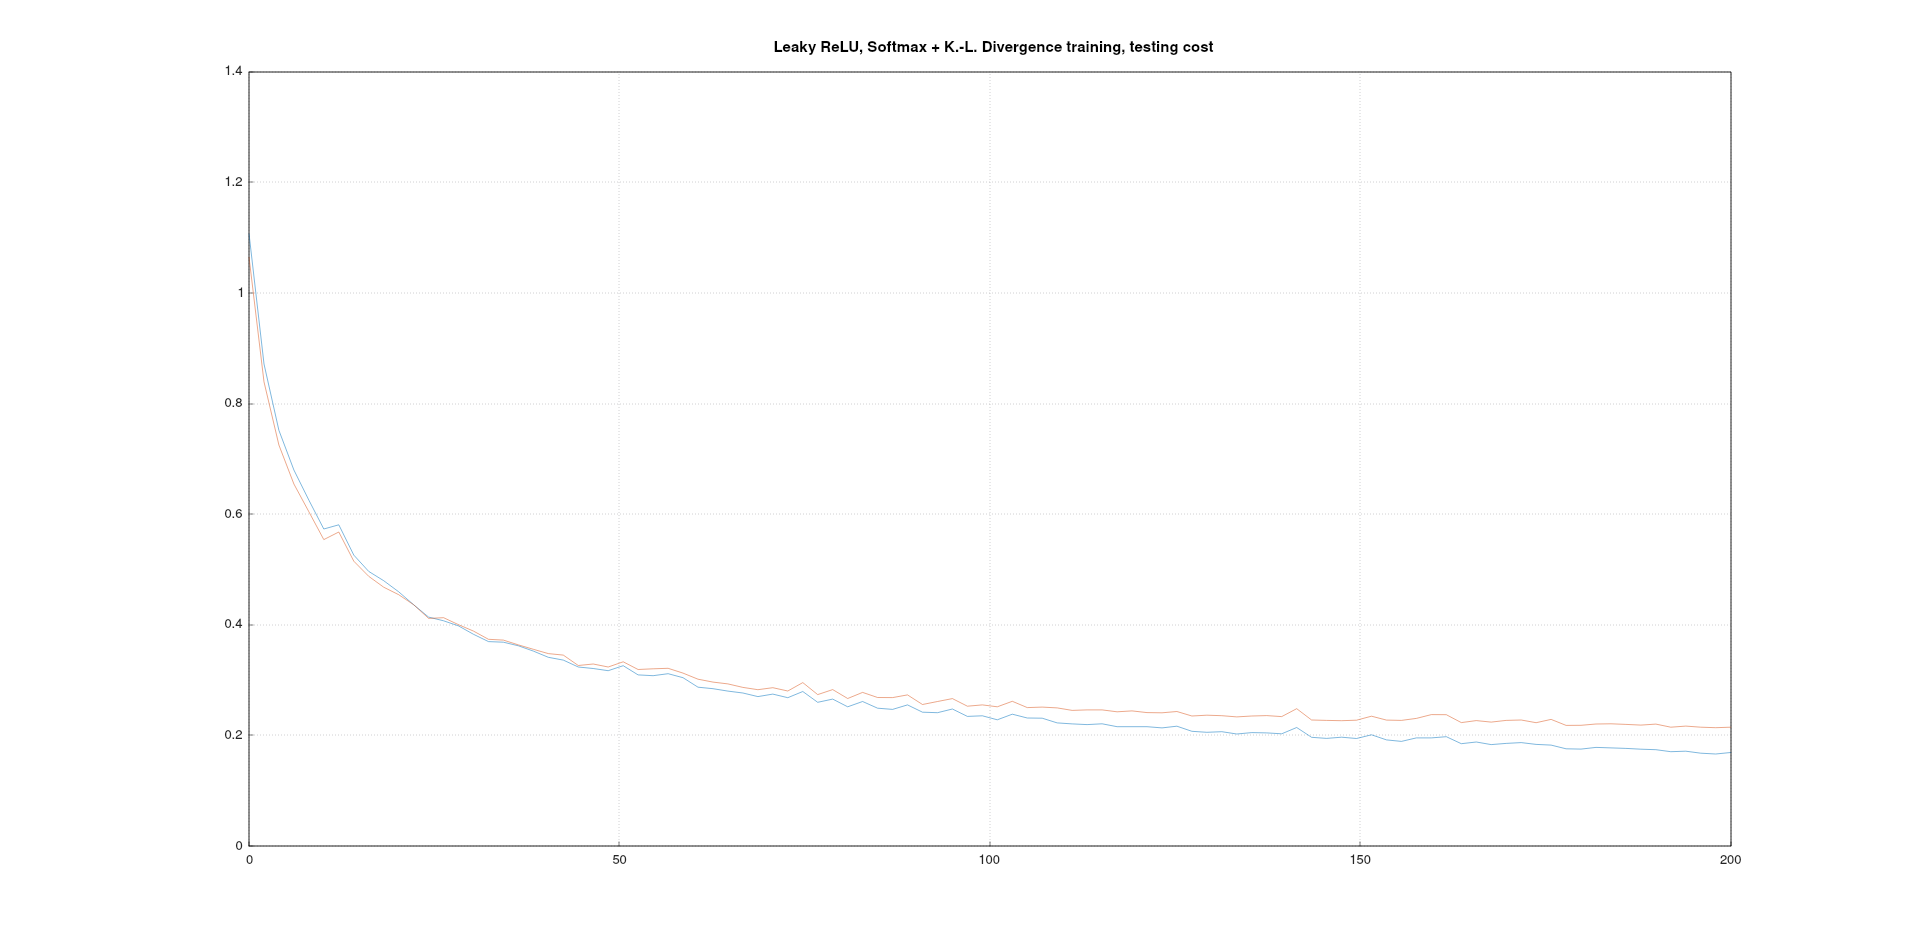
\includegraphics[width=\textwidth]{images/3_40_leaky_relu_softmax_kl_divergence_cost.png}
  \caption{}
  \label{fig:3_40_leaky_relu_softmax_kl_divergence_cost}
\end{figure}

На рисунке \ref{fig:3_40_leaky_relu_softmax_kl_divergence_accuracy} изображено изменение точности за период обучения персептрона.
В результате, точность на данных для обучения составляет $\frac{48315}{50000} \approx 96,63\%$, на тестовых данных --- $\frac{9457}{10000} = 94,57\%$.

\begin{figure}[!htb]
  \centering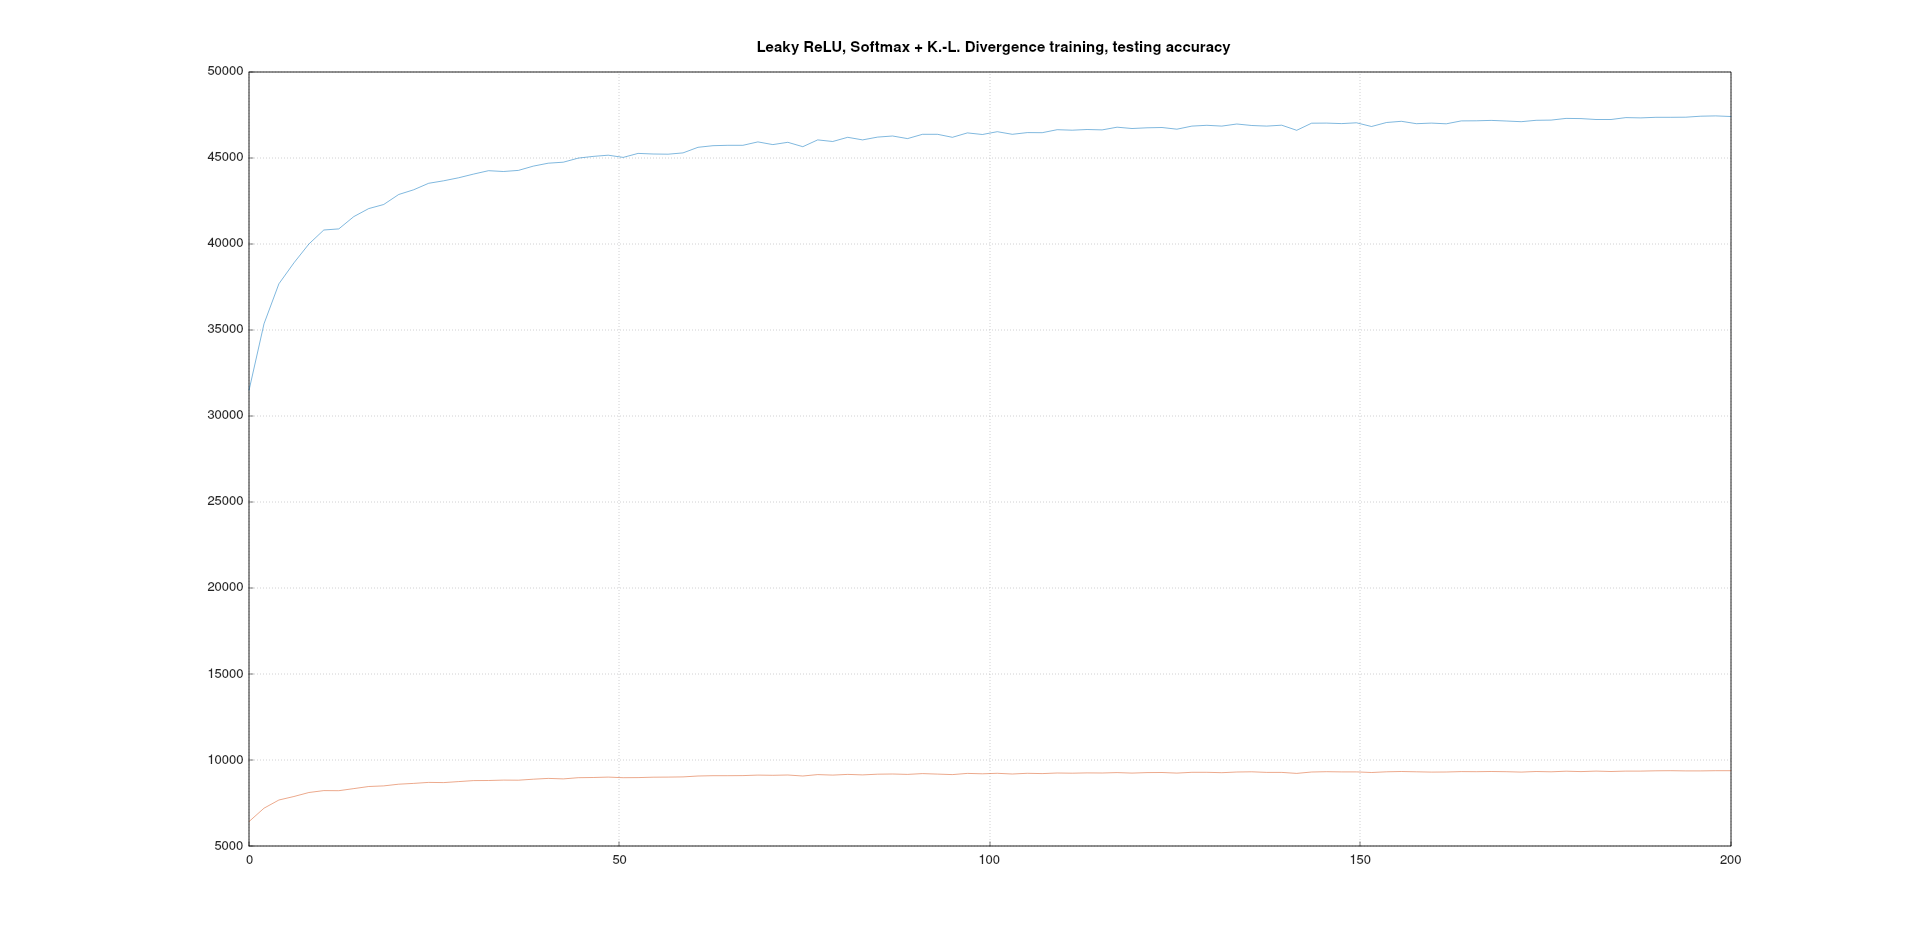
\includegraphics[width=\textwidth]{images/3_40_leaky_relu_softmax_kl_divergence_accuracy.png}
  \caption{}
  \label{fig:3_40_leaky_relu_softmax_kl_divergence_accuracy}
\end{figure}

\section{Вывод}

% 1x20
% Epoch 199; training cost: 0.166286; training accuracy: 47518/50000; testing cost: 0.193274; testing accuracy: 9421/10000;
% Epoch 199; training cost: 0.192402; training accuracy: 47194/50000; testing cost: 0.217352; testing accuracy: 9345/10000;
% Epoch 199; training cost: 0.17601; training accuracy: 47346/50000; testing cost: 0.201559; testing accuracy: 9415/10000;
%
% 1x40
% Epoch 199; training cost: 0.123245; training accuracy: 48121/50000; testing cost: 0.161724; testing accuracy: 9527/10000;
% Epoch 199; training cost: 0.131022; training accuracy: 48097/50000; testing cost: 0.173189; testing accuracy: 9483/10000;
% Epoch 199; training cost: 0.118821; training accuracy: 48233/50000; testing cost: 0.168346; testing accuracy: 9506/10000;
%
% 3x20
% Epoch 199; training cost: 0.163502; training accuracy: 47504/50000; testing cost: 0.206251; testing accuracy: 9416/10000;
% Epoch 199; training cost: 0.157613; training accuracy: 47681/50000; testing cost: 0.216353; testing accuracy: 9386/10000;
% Epoch 199; training cost: 0.163792; training accuracy: 47487/50000; testing cost: 0.213412; testing accuracy: 9369/10000;
%
% 3x40
% Epoch 199; training cost: 0.105351; training accuracy: 48422/50000; testing cost: 0.190718; testing accuracy: 9481/10000;
% Epoch 199; training cost: 0.118457; training accuracy: 48232/50000; testing cost: 0.17582; testing accuracy: 9502/10000;
% Epoch 199; training cost: 0.111865; training accuracy: 48315/50000; testing cost: 0.197848; testing accuracy: 9457/10000;

Исходя из полученных результатов видно, что наименьшая ошибка на тестовых данных достигается при наличии 1-го скрытого слоя с 40 нейронами: для
среднеквадратичной функции, перекрёстной энтропии, дивергенции Кульбака-Лейблера точность на тестовых данных составляет $95,27\%$, $94,83\%$ и $95,06\%$
соответственно. Увеличение числа нейронов в скрытых слоях может способствовать уменьшению ошибки и повышению точности персептрона.

При 3-х скрытых слоях с 40 нейронами ошибка на данных для обучения меньше, чем в предыдущем случае, однако ошибка на тестовых данных выше --- это может
свидетельствовать о переобучении персептрона; более простая архитектура сети (с 1-м скрытым слоем, а не 3-мя) показывает лучший результат.

Между конфигурациями, где скрытые слои содержат по 20 нейронов, особенных различий нет; здесь ошибка в целом выше, чем в предыдущих двух случаях.

\end{document}
